\documentclass[11pt, a4paper]{article}
\usepackage[margin=1in, top=1.5in, bottom=1.5in]{geometry}
\usepackage{subcaption}
\usepackage{graphicx}
% \usepackage{subfigure}
\usepackage{float}
\usepackage{titlesec}
\usepackage{amsmath}
\usepackage{amssymb}
\usepackage{amsthm}
\usepackage{cases}
\usepackage[english]{babel}
\usepackage{hyperref}
\usepackage{enumitem}
\usepackage{authblk}
\usepackage{dsfont}
\usepackage{sectsty}
\usepackage{xcolor}

\usepackage{todonotes}
\providecommand{\MH}[1]{\todo[inline,author={MH},color=red!20!white]{#1}}
\providecommand{\MT}[1]{\todo[inline,author={MT},color=blue!20!white]{#1}}
\providecommand{\RM}[1]{\todo[inline,author={RM},color=green!20!white]{#1}}

% THEOREM / PROPOSITIONS / LEMMAS etc...

\theoremstyle{break}
	\newtheorem{thm}{Theorem}[section]
\theoremstyle{break}
    \newtheorem{prp}{Proposition}[section]
\theoremstyle{break}
	\newtheorem{asm}{Assumption}[section]
\theoremstyle{break}
	\newtheorem{rem}{Remark}[section]
\theoremstyle{break}
	\newtheorem{lem}{Lemma}[section]
\theoremstyle{break}
	\newtheorem{cor}{Corollary}[section]
    \theoremstyle{break}
	\newtheorem{con}{Conclusion}[section]
\theoremstyle{break}
	\newtheorem{defi}{Definition}[section]
\theoremstyle{break}
	\newtheorem{expe}{Experiment}[section]
\theoremstyle{break}
    \newtheorem{main_contrib}{Contribution}

% USEFUL COMMANDS

% writing - labels
\makeatletter
\newcommand{\mylabel}[2]{#2\def\@currentlabel{#2}\label{#1}}
\makeatother

\providecommand{\keywords}[1]
{
  \small	
  \textbf{\textit{Keywords}} #1
}

% objects
\newcommand{\Leo}{\mathcal{L}_{\varepsilon}}
\newcommand{\Seq}[2]{\left\{#1_#2\right\}_{#2 = 0}^\infty}

% spaces
\newcommand{\Leb}{L^2\left(\Omega\right)}
\newcommand{\Lei}{L^\infty\left(\Omega\right)}
\newcommand{\CDR}{C^1\left(\mathbb{R}\right)}
\newcommand{\CCSRn}{C_c\left(\mathbb{R}^n\right)}

% operators

\DeclareMathOperator*{\argmax}{arg\,max}
\DeclareMathOperator*{\argmin}{arg\,min}
\DeclareMathOperator{\supp}{supp}
\DeclareMathOperator{\Ima}{Im}
\DeclareMathOperator{\divergence}{div}

\DeclareMathOperator{\Tr}{Tr}

\counterwithin{equation}{section}

\title{Extinction and persistence criteria in non-local Klausmeier model of vegetation dynamics on flat landscapes}



\author[c, a]{Maciej Tadej \thanks{Corresponding author. Email: maciej.tadej@math.uni.wroc.pl}}
\author[a, c]{Michael Hecht \thanks{Co-author. Email: m.hecht@hzdr.de}}
\author[a, b, d]{Ricardo Martinez-Garcia \thanks{Co-author. Email: r.martinez-garcia@hzdr.de}}

\affil[a]{\textit{Center for Advanced Systems Understanding (CASUS) -- Helmholtz-Zentrum
    Dresden-Rossendorf (HZDR), Untermarkt 20, G\"orlitz 02826, Germany}}
\affil[b]{\textit{ICTP South American Institute for Fundamental Research \& Instituto de F\'isica Te\'orica, Universidade
Estadual Paulista - UNESP, São Paulo SP, Brazil}}
\affil[c]{\textit{Institute of Mathematics, University of Wrocław, pl. Grunwaldzki 2, 50-384 Wrocław, Poland}}
\affil[d]{\textit{Department of Ecology, Institute of Biosciences, University of S\~ao Paulo, S\~ao Paulo, R. do Mat\~ao, 321 - Butant\~a, 05508-090 , S\~ao Paulo, Brazil}}

\date{}

\begin{document}

\maketitle

\hspace{20pt}

\begin{abstract}
    This paper investigates the dynamics of vegetation patterns in water-limited ecosystems using a generalized Klausmeier model that incorporates non-local plant dispersal within a finite habitat. We establish the well-posedness of the system and provide a rigorous analysis of the conditions required for vegetation survival. Our results identify a critical patch size governed by the trade-off between local growth and boundary losses; habitats smaller than this threshold lead to inevitable extinction. Furthermore, we derive a critical maximal biomass density below which the population collapses to a desert state, regardless of the domain size. We determine stability criteria for stationary solutions and describe the emergence of stable, non-trivial biomass distributions. Numerical experiments comparing sub-Gaussian and super-Gaussian kernels confirm that non-local dispersal mechanisms, particularly those with fat tails, enhance ecosystem resilience by allowing vegetation to persist in smaller, fragmented habitats than predicted by classical local diffusion models.
\end{abstract}

\begin{keywords}
non-local dispersal, vegetation patterns, critical patch size, Klausmeier model, reaction-diffusion systems, finite habitat
\end{keywords}

\newpage

\section{Introduction}

Water-limited ecosystems often exhibit a variety of regular vegetation patterns \cite{Rietkerk2008,Tarnita2024,Martinez-Garcia2022} resulting from the interplay between various water-vegetation feedbacks acting at different scales \cite{Borgogno2009,Martinez-Garcia2014,Meron2018}. Importantly, these patterns often form in response to increasingly harsh conditions and can therefore be important for ecosystem survival and persistence \cite{Meron2016}. Due to the long time scales at which vegetation patterns form and change, mathematical modeling has been an essential tool to better understand how patterns form and how they affect ecosystem dynamics \cite{Meron2016,Martinez-Garcia2023}. 

Different modeling efforts have, for example, suggested that pattern shapes could be used as early indicators of impending desertification processes, as water-stressed vegetation consistently forms hexagonally distributed spots in hyper-arid conditions \cite{Lefever1997,VonHardenberg2001,Meron2004,Rietkerk2002}. More recent results indicate that patterns could alternatively enhance ecosystem resilience by allowing ecosystems to avoid sudden collapses through spatial reshaping of the vegetation cover \cite{Rietkerk2021}. Mathematical modeling has thus made key contributions to our understanding of self-organization in water-limited ecosystems. However, most of these models are formulated in ideal conditions, assuming infinite domains, and thus neglecting how more realistic boundary conditions could change both spatial patterns and vegetation survival (but see, e.g., \cite{Clerc2021,PintoRamos2023,PintoRamos2025}).

In less applied scenarios, researchers have studied population dynamics in bounded domains, mainly using extensions of the Fisher–KPP equation \cite{Cantrell1999,Fagan2009,Colombo2018,Dornelas2024} known as KISS \textcolor{blue}{(Kierstead–Slobodkin–Skellam)} models in the mathematical biology literature \cite{Skellam1951,Kierstead1953}. KISS models show that population survival in confined domains---or habitats in ecological terms---requires that the domain is large enough so that reproduction within the domain balances population loss due to density fluxes through the domain edges \cite{Cantrell2004}. For domains smaller than this critical size, population extinction is the only stable solution. A key difference between these studies and vegetation-pattern models is that the latter often present non-local terms that account for long-range processes responsible for vegetation growth (e.g., resource intake via roots or sibling dispersal \cite{Martinez-Garcia2014,Eigentler2018}). Therefore, models for vegetation pattern formation provide an ideal scenario to extend KISS models to cases in which population dynamics are spatially non-local. 

We investigate the relationship between non-local population dynamics in finite habitats and population survival. To establish this connection, we use a generalized formulation of Klausmeier's model for vegetation pattern formation in flat landscapes that accounts for non-local plant dispersal \cite{Eigentler2018,Klausmeier1999}. We extend this formulation to consider the more realistic case in which vegetation can only grow in a finite region that is always surrounded by a hostile environment. Regarding our approach, we found several interesting results. Namely, in \cite{JaramilloMeraz2024,CappaneraJaramilloWard2024} the authors constructed weak, local-in-time solutions. In a similar framework, though not involving the water density effects directly, the authors have shown several important properties such as large-time asymptotics, existence of non-trivial stable patterns, and a critical domain size, see \cite{Tadej2025,BaiLiWang2025,ReimerBonsallMaini2015,Sun2023} and references therein. When the local diffusion of water is replaced by a non-local operator it is known that there is a unique, global-in-time solution \cite{LaurencotWalker2023}.

\subsection{The non-local Klausmeier model}

The \textcolor{blue}{modified Klausmeier model} for vegetation patterns describes the coupled dynamics of the vegetation biomass $v := v(x,t)$ and the water concentration $w := w(x,t)$ as a non-linear reaction-diffusion system. 
Here, we extend the dimensionless form \cite{Eigentler2018} to the finite habitat case 
\begin{numcases}{}
    v_t = d_v\mathcal{L} v + v^2 w - B v & \hspace{2mm} $(x, t) \in \Omega \times [0, T],$ \label{eq:u} \\
    w_t = d_w\Delta w - v^2w - w + A & \hspace{2mm} $(x, t) \in \Omega \times [0, T],$ \label{eq:v} \\
    v = 0 & \hspace{2mm} $(x,t) \in \mathbb{R}^n \setminus \Omega  \times [0,T], $ \label{eq:u_bound} \\
    w = 0 & \hspace{2mm} $(x,t) \in \partial\Omega \times [0,T],$ \label{eq:v_bound} \\
    v(0) = v_0 & \hspace{2mm} $x \in \Omega ,$ \label{eq:Unit} \\
    w(0) = w_0 & \hspace{2mm} $x \in \Omega\,, $ \label{eq:v_init}
\end{numcases}
where $T > 0$ is the evolution time, $\Omega \subset \mathbb{R}^n$ an open and bounded domain, 
 $d_v > 0$ models plant dispersal, $d_w > 0$ the water diffusion, $A > 0$ the average rainfall, and $B > 0$ the mortality. 

\textcolor{blue}{Several empirical studies show that local diffusion is not sufficient to capture vegetation spread through seed dispersal. Seed dispersal, whether mediated by wind or animals (e.g., frugivores), produces fat-tailed, leptokurtic dispersal kernels \cite{MoralesCarlo2006, SnellEtAl2019}. For example, the interaction between animal foraging movements and varying seed gut passage times results in dispersal patterns characterized by a sharp peak near the parent plant and a fat tail accounting for long-distance dispersal events \cite{MoralesCarlo2006}. Furthermore, empirical tracking of frugivorous birds confirms that natural variations in animal movement generate fat-tailed population-level kernels, significantly increasing the probability of long-range seed deposition compared to standard random-walk approximations \cite{SnellEtAl2019}. Finally, we want to highlight that another kind of dispersal kernels might arise due to the secondary dispersal phenomenon, for instance when animals feed seeds from fallen fruits rather then the plant itself. In this case it might be appropriate to use skewed dispersal kernels, for instance see \cite{SallyGabriel2009, ConsoloValenti2019}. Motivated by these empirical findings, we consider a general non-local dispersal operator $\mathcal{L}$, given as}
\begin{equation}
    \label{eq:DispersalOperatorDefinition_1}
    \mathcal{L} v(x) = \mathds{1}_{\Omega}(x)\int_{\mathbb{R}^n} J(x-y)\left(v(y) - v(x)\right)\:dy\,.
\end{equation}
Here, $\mathds{1}_\Omega$ is the characteristic function of the domain $\Omega$ and $J : \mathbb{R}^n \rightarrow \mathbb{R}_{\geq 0}$ is an integral kernel fulfilling the assumptions listed below.

\begin{asm}
\label{assumptions_general_kernel}
We assume the integral kernel $J \in C^0(\mathbb{R}^n)$ satisfies the following properties:
\begin{enumerate}[label=\textnormal{(\arabic*)}, leftmargin=2em]
    \item[\mylabel{J1}{(J1)}] \textbf{Positivity:} 
    $J(z) \geq 0$ for all $z \in \mathbb{R}^n$, and $J(0) > 0$. 

    \item[\mylabel{J2}{(J2)}] \textbf{Symmetry:} 
    $J(z) = J(-z)$ for all $z \in \mathbb{R}^n$. 

    \item[\mylabel{J3}{(J3)}] \textbf{Decay:} 
    $J(z) \to 0$ as $|z| \to \infty$. 

    \item[\mylabel{J4}{(J4)}] \textbf{Finite second moment:} $\int_{\mathbb{R}^n} J(z)\,|z|^2 \,dz < \infty.$

    \item[\mylabel{J5}{(J5)}] \textbf{Normalization:} $\int_{\mathbb{R}^n} J(z)\,dz = 1.$
\end{enumerate}
\end{asm}

Assumption \ref{J5} and the non-local Dirichlet boundary condition \eqref{eq:u_bound} allow us to rewrite \eqref{eq:DispersalOperatorDefinition_1} as
\begin{equation}
    \label{EQ:DispersalOperatorDefinition_2}
    \mathcal{L} v(x) = \mathds{1}_{\Omega}(x) \left(\int_{\Omega} J(x-y) v(y)\:dy - v(x)\right).
\end{equation}

We furthermore impose the following constraints on the domain $\Omega$.

\begin{asm}
\label{assumptions_domain}
We assume that $\Omega \subset \mathbb{R}^n$ is bounded, open and satisfies the following properties:
\begin{enumerate}[label=\textnormal{(\arabic*)}, leftmargin=2em]
    \item[\mylabel{O1}{(O1)}] \textbf{Uniform estimates:} 
    Let $\{\phi_j\}_{j \in \mathbb{N}}$ be the eigenfunctions of $\Delta$ with Dirichlet boundary conditions. There exists a constant $C := C(\Omega) > 0$ such that $\sup_{j \in \mathbb{N}}\|\phi_j\|_\infty \leq C$.

    \item[\mylabel{O2}{(O2)}] \textbf{Boundary regularity:} 
    The boundary of $\Omega$ is sufficiently regular, i.e.\ $\partial\Omega \in C^k$ with suitable $k \in \mathbb{N}$.
\end{enumerate}
\end{asm}

\textcolor{blue}{We point out that here we consider a specific, non-local Dirichlet boundary condition given by equation \eqref{eq:u_bound}. This is a non-local analogue of the standard Dirichlet boundary condition. As we assumed that $v = 0$ in $\mathbb{R}^n \setminus \Omega$, it means that we are considering the domain surrounded by hostile environment, creating the boundary loss of vegetation due to transport outside of the domain $\Omega$. One could consider even more realistic case where $v = g(x)$ in  $\mathbb{R}^n \setminus \Omega$, however this would alter analysis of our problem, due to appearance of inhomogeneous reaction terms. We refer our reader to \cite{MolinoRossi2016} and references therein for more informations on this subject.}

\subsection{Main results}

Here, we briefly summarize how our theoretical and numerical results contribute to the field of theoretical ecology.

\begin{main_contrib}[Critical Patch Size and Kernel Shape]
\label{contrib:main_contrib_cps_ks}
We derive an analytical criterion for vegetation persistence based on the spectral properties of the dispersal operator. Specifically, as shown in Theorem \ref{thm:critical_patch_size}, extinction is guaranteed if the dispersal rate $d_v$ exceeds a threshold $M/\beta_1$, where $M$ is related to the maximum growth rate and $\beta_1$ is the principal eigenvalue of the operator $-\mathcal{L}$ on $\Omega$. Since $\beta_1$ scales inversely with the domain size (see Theorem \ref{thm:critical_patch_size}), this establishes a \textit{critical patch size} for persistence. 

Crucially, our numerical analysis reveals that this critical size is sensitive to the shape of the dispersal kernel. We show that non-local kernels with heavier tails (i.e., higher kurtosis) significantly reduce the critical patch size compared to the classical Laplacian diffusion (see Figure \ref{fig:critical_patch_size}, left panel). This implies that long-range dispersal mechanisms enhance ecosystem resilience in fragmented landscapes.
\end{main_contrib}

\textcolor{blue}{In accordance to Contribution \ref{contrib:main_contrib_cps_ks}, note that, with fixed dispersal kernel, smaller and smaller patch sizes easily translate into boundary losses. This boundary losses are directly connected with the principle eigenvalue driving the critical patch size criterion, see Theorem \ref{thm:critical_patch_size} and equation \eqref{eq:d_v_condition_1}. We acknowledge that for animal movement in small habitat, this might be irrelevant, as animals adapt movement patterns to habitat availability, but one can find other examples driven by other modes of dispersal, such as wind.}

\begin{main_contrib}[Minimum Biomass Threshold for Persistence]
We identify a critical threshold for the initial biomass density required to prevent ecosystem collapse. Our stability analysis, formalized in Theorem \ref{thm:Exinction-Of-Vegetation}, demonstrates that if the maximal biomass density drops below a critical level, approximately scaled by the ratio of mortality to rainfall, $\|V\|_\infty \sim B/A$, then the system is attracted to the trivial desert state regardless of the habitat size. This theoretical lower bound is numerically confirmed by the bifurcation diagrams in Figures \ref{fig:bifurcation_diagram_slow} and \ref{fig:bifurcation_diagram_fast}, which show that no stable non-trivial solutions exist below this biomass threshold.
\end{main_contrib}

\begin{main_contrib}[Existence and Stability of Quasi Uniform Solutions]
We prove the existence of stable, non-trivial stationary solutions $V(x)$ that bifurcate from the spatially uniform states of the kinetic system.
\begin{itemize}
    \item \textcolor{blue}{\textbf{Existence Condition (Quasi Uniform States):} While the algebraic threshold $A > 2B$ is a well-known requirement for the existence of uniform vegetation in infinite domains (the kinetic saddle-node bifurcation), our setting considers a finite habitat surrounded by a hostile environment ($v=0$). The mathematical novelty here lies in rigorously proving that, due to the finite domain and non-local boundary conditions, stationary localized patches persist over a continuous parameter range. Under the bounds established in Proposition \ref{prp:nonlinearity_f_properties_at_v_star}, Theorem \ref{thm:Stationary-Solutions-Existence} mathematically guarantees the existence of these non-trivial, localized stationary solutions exactly up to the kinetic tipping point $A = 2B$.}
    \item \textbf{Stability Regime:} By analyzing the linearized operator in Theorem \ref{thm:Stationary-Solutions-Stability}, we show that these spatially structured solutions are linearly exponentially stable, provided that the transport parameters $d_v$ and $d_w$ are sufficiently small.
\end{itemize}
Unlike the classical reaction-diffusion model, which predicts smooth profiles, the non-local model supports stable solutions characterized by sharp biomass gradients at the habitat boundaries (as visualized in the right panel of Figure \ref{fig:critical_patch_size}), offering a distinct morphological signature of non-local interactions.
\end{main_contrib}


\subsection{Structure}
The remainder of this article is organized as follows. 
In Section 2, we establish the well-posedness of the non-local Klausmeier model by proving the local-in-time existence and uniqueness of solutions to the problem \eqref{eq:u}-\eqref{eq:v_init}. We also demonstrate fundamental properties such as the non-negativity of solutions and the existence of an invariant region. 
Section 3 contains the core mathematical analysis of this paper, where we provide a rigorous proof for the existence of non-trivial stationary solutions. 
In Section 4, we investigate the long-term behavior of these solutions by deriving criteria for both the extinction of vegetation and the persistence of these equilibria through a stability analysis. 
Section 5 is devoted to numerical experiments designed to validate and illustrate our theoretical findings. We present two main computational studies: the first investigates the critical patch size for different dispersal kernels, while the second explores the system's bifurcation structure. 
Finally, in Section 5.1, we summarize our main conclusions and outline potential directions for future research.

\section{Existence of solutions}
In order to show that the non-local Klausmeier model \eqref{eq:u}--\eqref{eq:v_init} is well-posed we start by constructing local-in-time solutions. 

\subsection{Local-in-time solutions} 
We denote with 
\begin{equation}
    \label{EQ:C_0_OMEGA}
    C_{0, \Omega}(\mathbb{R}^n) = \left\{ v \in L^\infty(\mathbb{R}^n): v \in C^0(\Omega), \: v = 0 \text{ in } \mathbb{R}^n \setminus \Omega \right\},
\end{equation}
the space of functions vanishing outside of $\Omega$, which becomes a Banach space when equipped with the norm $\|v\|= \|v\|_{C^0(\Omega)} + \|v\|_{L^\infty(\mathbb{R}^n\setminus \Omega)}$. We study the linear part in the vegetation equation \eqref{eq:u}.  

\begin{lem} 
Let $\mathcal{L}:  C_{0, \Omega}(\mathbb{R}^n) \to C_{0, \Omega}(\mathbb{R}^n)$ be the non-local dispersal operator from equation~\eqref{eq:DispersalOperatorDefinition_1}, $B>0$.
Consider the linear operator $\mathcal{A}: C_{0, \Omega}(\mathbb{R}^n) \to C_{0, \Omega}(\mathbb{R}^n)$ given as
\begin{align}
    \label{EQ:A_OPERATOR_DEFINITION}
    \mathcal{A} v (x) =
    \begin{cases}
        d_v\mathcal{L}v - Bv &x \in \Omega, \\
        0 &x \in \mathbb{R}^n \setminus \Omega,
    \end{cases} \quad d_v >0 \,.
\end{align} 
We denote with $\mathcal{T}(t) : C_{0, \Omega} (\mathbb{R}^n) \to  C_{0, \Omega} (\mathbb{R}^n)$, $t \geq 0$, the solution operator of the linear problem 
    \begin{equation}
        \label{eq:v_semilinear_problem}
        \frac{d}{dt} v(t) = \mathcal{A} v (t) \,, \quad t > 0 \,, \quad  v(0) = v_0 \in C_{0, \Omega}.
    \end{equation}
Then $\mathcal{T}(t) = e^{t\mathcal{A}}$ is well defined and the family $\{\mathcal{T}(t)\}_{t \geq 0}$ is a uniformly continuous semigroup of contractions.
    \label{lem:A_SEMIGROUP_GENERATOR}
\end{lem}

\begin{proof} 
    First, observe that by definition of $\mathcal{L}$, the operator $\mathcal{A}$ is bounded and linear. For each $v \in C_{0, \Omega}$ the solution of the problem \eqref{eq:v_semilinear_problem} exists for all $t \geq 0$, it is unique and given explicitly by $u(t) = \mathcal{T}(t)u(0)$, with $\mathcal{T}(t) = e^{t\mathcal{A}} = \sum_{n=1}^\infty \frac{\mathcal{A}^n t^n}{n!}$. Hence, $\mathcal{T}(t)$ is well defined and $\{\mathcal{T}(t)\}_{t \geq 0}$ is a uniformly continuous semigroup, see \cite[Proposition 1.2.2]{cazenave1998introduction} and \cite[Theorem 1.2]{Pazy}. Thanks to  \cite[Proposition 3.2]{ChasseigneChavesRossi2006} and \cite[Theorem 2.1]{Tadej2025}, the spectrum of the operator $\mathcal{L}$ is discrete and negative. Thus, for each $t \geq 0$, $\mathcal{T}(t):  C_{0, \Omega}(\mathbb{R}^n) \rightarrow C_{0, \Omega}(\mathbb{R}^n)$ is a contraction \cite[Proposition V.1.7]{EngelNagel2000}.    
\end{proof}

Next we study the water equation \eqref{eq:v}. Denote by $C_0(\Omega)$ the Banach space of functions continuous in $\overline{\Omega}$ and vanishing on $\partial\Omega$.

\begin{lem}
    \label{lem:B_SEMIGROUP_GENERATOR}
    Consider the linear operator $\mathcal{B}: D(\mathcal{B}) \to C_0(\Omega)$ given by 
    \begin{align}
        \label{EQ:B_OPERATOR_DEFINITION}
        \mathcal{B} w (x) = 
        \begin{cases}
            d_w \Delta w - w &x \in \Omega, \\
            0 &x \in \partial \Omega, 
        \end{cases} \quad d_w > 0 \,, 
    \end{align}
    where the domain $D(\mathcal{B})$ is given by
    \begin{equation}
        \label{EQ:B_DOMAIN_DEFINITION}
        D(\mathcal{B}) = \left\{ w \in C^2_0(\Omega): \Delta w \in C_0(\Omega) \right\}\,.
    \end{equation}
    Then the solution operator $\mathcal{T}(t): D(\mathcal{B}) \to C_0(\Omega)$ given by $\mathcal{T}(t) = e^{t\mathcal{B}}$ is well defined and the family $\{\mathcal{T}(t)\}_{t \geq 0}$ is a strongly continuous semigroup of contractions.
\end{lem}
\begin{proof}
    The proof can be found in  \cite[Theorem 6.1.8]{Arendt2001}.
\end{proof}
We use the ingredients above to construct the local-in-time solutions of the Klausmeier system.
\begin{thm}
    \label{thm:Well-Posedness}
    Let $(v_0, w_0) \in C_{0, \Omega}(\mathbb{R}^n) \times C_0(\Omega)$. Then there exists $0 < T := T(v_0, w_0)$ and a unique solution $(v, w)$ to the problem \eqref{eq:u}--\eqref{eq:v_init}, such that
    \begin{equation}
        v \in C\left([0, T], C_{0, \Omega}(\mathbb{R}^n)\right) \cap C^1\left([0, T), C_{0, \Omega}(\mathbb{R}^n)\right),
    \end{equation}
    and
    \begin{equation}
        w \in C\left([0, T], C_0(\Omega)\right) \cap C^1\left([0, T), C_0(\Omega)\right).
    \end{equation}
\end{thm}
\begin{proof}
    Given $\mathcal{A}, \mathcal{B}$ by the formulas \eqref{EQ:A_OPERATOR_DEFINITION} and \eqref{EQ:B_OPERATOR_DEFINITION}--\eqref{EQ:B_DOMAIN_DEFINITION} respectively, let us define the operator $\mathcal{C}: C_{0, \Omega}(\mathbb{R}^n) \times D(\mathcal{B}) \to C_{0, \Omega}(\mathbb{R}^n) \times C_0(\Omega)$ as follows
    \begin{equation}
        \mathcal{C} = 
        \begin{bmatrix}
            \mathcal{A} & 0\\ 0 & \mathcal{B}
        \end{bmatrix}.
    \end{equation}
    Next, denote the vectors $u = (v, w)$ and $u_0 = (v_0, w_0)$. Using this notation we rewrite the Klausmeier system \eqref{eq:u}--\eqref{eq:v_init} as
    \begin{equation}
        \label{eq:ClassicalSemigroupFormulation}
         u'(t) = \mathcal{C} u(t) + F(u(t)), \quad u(0) = u_0,
    \end{equation}
    where  $F: C_{0, \Omega}(\mathbb{R}^n) \times C_0(\Omega) \to C_{0, \Omega}(\mathbb{R}^n) \times C_0(\Omega)$ is given by
    \begin{align}
        F(u) = F(v, w) = 
        \begin{cases}
            (v^2 w, -v^2 w + A) &x \in \Omega, \\
            (0, 0) &x \notin \Omega
        \end{cases}.
    \end{align}
    Lemma \ref{lem:A_SEMIGROUP_GENERATOR} and Lemma \ref{lem:B_SEMIGROUP_GENERATOR} yield that $\mathcal{C}$ generates a semigroup $\{\mathcal{T}(t)\}_{t \geq 0}$ of contractions on $C_{0, \Omega}(\mathbb{R}^n) \times C_0(\Omega)$. Thus, we construct the solution $u$ using the Duhamel formula \cite[Lemma 4.1.1]{cazenave1998introduction}
    \begin{equation}
        \label{eq:MildSemigroupFormulation}
         u(t) = \mathcal{T}(t) u_0 + \int_0^t \mathcal{T}(t-s) F(u(s)) \:ds.
    \end{equation}
    Since $u_0 \in C_{0, \Omega}(\mathbb{R}^n) \times C_0(\Omega)$ and $F$ is a locally Lipschitz function, we proceed with a standard Banach fixed point argument \cite[Proposition 4.3.3]{cazenave1998introduction}, ensuring that there exists a positive number $T := T(u_0)$ such that \eqref{eq:MildSemigroupFormulation} admits a unique solution $u \in C\left([0, T], C_{0, \Omega}(\mathbb{R}^n) \times C_0(\Omega)\right)$. To show differentiability in time one needs to integrate equations \eqref{eq:u}, \eqref{eq:v} to find that $u$ satisfies
    \begin{equation}
        \label{eq:IntegralFormula}
        u(t) = u_0 + \int_0^t (\mathcal{C}u(s) + F(u(s))) \:ds.
    \end{equation}
    Hence, the continuity of $u$ implies differentiability of $u$ in the time interval $[0, T)$.
\end{proof}
Given that solutions exist we continue by studying their properties. 

\subsection{Non-negative and bounded solutions} 
We start by showing the non-negativity and the existence of an invariant region $\Gamma$ for the system \eqref{eq:u}--\eqref{eq:v_init}.
\begin{thm}
    \label{thm:Non-negativity}
     Let the initial datum $(v_0, w_0) \in C_{0, \Omega}(\mathbb{R}^n) \times C_0(\overline{\Omega})$ be non-negative. Then the solution $(v, w)$ ensured by Theorem \ref{thm:Well-Posedness} is non-negative and for all $(x, t) \in \Omega \times [0, T]$ it holds
     \begin{equation}
         w(x,t) \leq \max\{\|w_0\|_\infty, A\} =: R_1 >0\,.
     \end{equation}
     Moreover, let $\Gamma = [0, B/R_1]$. If  $v_0(x) \in \Gamma$ for all $x \in \Omega$ then for all $(x, t) \in \Omega \times [0, T]$ the solution $v(x,t) \in \Gamma$.
\end{thm}
\begin{proof}
    It follows from the parabolic maximum principle that for all $(x, t) \in \Omega \times [0, T)$ we have the estimate of the form
    \begin{equation}
        \label{EQ:AprioriEstimate_V}
        0 \leq w(x, t) \leq \max\{\|w_0\|_\infty, A\} =: R_1.
    \end{equation}
    Next, we define the point $\xi := \xi(t) \in \Omega$ and evaluation $\mu := \mu(t)$ such that 
    \begin{equation*}
        \mu(t) := v(\xi(t), t) = \min_{x \in \Omega} v(x, t).
    \end{equation*}
    Without loss of generality, we take arbitrary $0 < s < t < T$ and use the 
    Lipschitz continuity of $\mu$ to estimate
    \begin{equation*}
        \left|\mu(t) - \mu(s)\right| \leq \left|v(\xi(s), t) - v(\xi(s), s)\right| \leq \max_{(x, r) \in \Omega \times [0, T]} |v(x, r)|\, |t-s|.
    \end{equation*}
    It follows from the Radamacher Theorem \cite[Theorem 3.2]{EvansGariepy2015} that $\mu$ is differentiable almost everywhere in $[0, T]$. Next, we estimate the difference quotients by applying the mean value theorem
    \begin{align*}
        \frac{\mu(t+h) - \mu(t)}{h} &\leq \frac{v(\xi(t+h), t+h) - v(\xi(t + h), t)}{h} = v_t(\xi(t + h), c(t, h)), \\
        \frac{\mu(t+h) - \mu(t)}{h} &\geq \frac{v(\xi(t), t+h) - v(\xi(t), t)}{h} = v_t(\xi(t), c(t, h)),
    \end{align*}
    where $c(t,h) \in [t, t+h]$ is an intermediate point. Passing with $h \rightarrow 0$, estimating $\mathcal{L}$ in a minimum point and using non-negativity of $w$, we obtain the differential inequality
    \begin{align}
        \label{eq:differential_inequality_min}
        \begin{split}
            \mu'(t) &= d_v \mathcal{L} v(\xi(t), t) + \mu^2(t) w(\xi(t), t) - B \mu(t) \geq - B \mu(t), \\
            \mu(0) &= \min_{x \in \Omega} v_0(x) \geq 0.
        \end{split}
    \end{align}
    When solved, inequality \eqref{eq:differential_inequality_min} yields the following lower bound 
    \begin{equation*}
        v(x,t) \geq \mu(t) \geq \mu(0) e^{-B t} \geq 0.
    \end{equation*}
    Now, we define the point $\zeta := \zeta(t) \in \Omega$ and evaluation $\nu := \nu(t)$ such that
    \begin{equation*}
        \nu(t) := v(\zeta(t), t) = \max_{x \in \Omega} v(x,t).
    \end{equation*}
    Proceeding as previously, we arrive at the following differential inequality
    \begin{align}
        \label{eq:differential_inequality_max}
        \begin{split}
            \nu'(t) &= d_v\mathcal{L} v(\zeta(t), t) + \nu^2(t) w(\zeta(t), t) - B \nu(t) \leq R_1 \nu^2(t) - B \nu(t), \\
            \nu(0) &= \max_{x \in \Omega} v_0(x) \leq B/R_1.
        \end{split}
    \end{align}
    When solved, inequality \eqref{eq:differential_inequality_max} yields the following upper bound
    \begin{equation}
        \label{EQ:AprioriEsitmate_Unvariant_Region}
        v(x,t) \leq \nu(t) \leq \frac{B\nu(0)}{R_1 \nu(0) + 
        (B - R_1 \nu(0)) e^{B t}} \leq B / R_1.
    \end{equation}
    Hence, $\Gamma = [0, B/R_1]$ is an invariant region.
\end{proof}
While so far we have focused on local-in-time solutions, we next study the long-time behavior of the Klausmeier system. In particular, we use the results above for the stability analysis of stationary solutions.  

\section{Stationary solutions}
We seek stationary solutions of the Klausmeier system \eqref{eq:u}--\eqref{eq:v_init}, i.e.\ solutions of the system  
\begin{numcases}{}
    0 = d_v \mathcal{L} v + v^2 w - B v & \hspace{2mm} $x \in \Omega,$ \label{eq:u_stationary} \\
    0 = d_w\Delta w - v^2w - w + A & \hspace{2mm} $x \in \Omega,$ \label{eq:v_stationary} \\
    v = 0 & \hspace{2mm} $x \in \mathbb{R}^n \setminus \Omega , $ \label{eq:u_bound_stationary} \\
    w = 0 & \hspace{2mm} $x \in \partial\Omega.$ \label{eq:v_bound_stationary}
\end{numcases}

We start by showing that there exist non-trivial stationary solutions with non-constant water profiles. 

\subsection{Existence of non-constant water profiles}

As a first step, we aim to reduce the number of equations in the Klausmeier system \eqref{eq:u_stationary}--\eqref{eq:v_bound_stationary}. 
 
\begin{lem}
    \label{lem:existence_of_inhomogeneous_elliptic_v}
    Let $v \in C(\Omega)$ be a given function. Then there exists a unique solution $W \in W^{1,2}_0(\Omega) \cap W^{2,2}_{loc}(\Omega)$ of equations \eqref{eq:v_stationary} and \eqref{eq:v_bound_stationary}. Moreover, we have that $\|W \|_\infty \leq A$, where $A >0$ is the average rainfall. 
\end{lem}
\begin{proof}
    The proof of the existence and uniqueness is standard, see for instance \cite[Theorem 8.9]{gilbarg2001elliptic}. The remaining estimate $\|W\|_\infty \leq A$ follows directly from the elliptic maximum principle, we refer to \cite[Chapter 3]{gilbarg2001elliptic}.
\end{proof}

Next we show that the mapping $W = W(v)$ is Lipschitz continuous.
\begin{lem}
    \label{lem:stationary_v_lipschitz_constant}
    Let $B_R \subset C(\Omega)$ be the closed ball of radius $R > 0$ centered at $0$. 
    Consider the map $W : B_R \rightarrow W^{1,2}_0(\Omega)$, with $W=W(v)$ being the solution of the problem \eqref{eq:v_stationary}, \eqref{eq:v_bound_stationary}. Then $W (B_R) \subset L^\infty(\mathbb{R}^n)$ and for arbitrary $v_1, v_2 \in B_R$ there holds
    \begin{equation}
        \|W(v_1) - W(v_2)\|_\infty \leq 2 A R \|v_1 - v_2\|_\infty.
    \end{equation}
\end{lem}

\begin{proof}
    For arbitrary $v_1, v_2 \in B_R \subset L^\infty(\Omega)$ we define the difference $u = W(v_1) - W(v_2)$, satisfying 
    \begin{align}
        \label{eq:Difference_ELLIPTIC_DEF}
        \begin{cases}
            d_w\Delta u - (v_1^2 + 1) W(v_1) + (v_2^2 + 1) W(v_2) = 0, &\quad x \in \Omega, \\
            u = 0, &\quad x \in \partial\Omega.
        \end{cases}
    \end{align}
    Since $W(v_1) = u + W(v_2)$, we can equivalently express problem \eqref{eq:Difference_ELLIPTIC_DEF} as
    \begin{align}
        \label{eq:lipschitz_continuity_formulation_difference}
        \begin{cases}
            d_w\Delta u - (v_1^2 + 1) u  = W(v_2) (v_1^2 - v_2^2), &\quad x \in \Omega, \\
            u = 0, &\quad x \in \partial\Omega.
        \end{cases}
    \end{align}
    We estimate the supremum norm of the right-hand side of the first equation in \eqref{eq:lipschitz_continuity_formulation_difference}
    \begin{equation}
        \label{eq:Linfty_norm_rhs_difference_estimate}
        \|W(v_2) (v_1^2-v_2^2)\|_\infty \leq 2AR\|v_1-v_2\|_\infty.
    \end{equation}
    Note that by Lemma \ref{lem:existence_of_inhomogeneous_elliptic_v} $u \in W^{1,2}(\Omega)$. Thus, by regularity theory \cite[Theorems 8.33 and 8.34]{gilbarg2001elliptic} and the bound \eqref{eq:Linfty_norm_rhs_difference_estimate} we obtain that the solution $u$ of the problem \eqref{eq:lipschitz_continuity_formulation_difference} satisfies
    \begin{equation}
        \|W(v_1) - W(v_2)\|_{C^{1, \alpha}(\Omega)} =: \|u\|_{C^{1, \alpha}(\Omega)}  \leq 2AR\|v_1-v_2\|_\infty,
    \end{equation}
    with $0 < \alpha < 1$. Finally, the definition of the norm $\|\cdot\|_{C^{1,\alpha}(\Omega)}$ implies that 
    \begin{equation}
        \|W(v_1) - W(v_2)\|_\infty = \|u\|_\infty \leq \|u\|_{C^{1, \alpha}(\Omega)}  \leq 2AR\|v_1-v_2\|_\infty.
    \end{equation}
\end{proof}
In light of the fact above, we consider the following system of constant solutions of equations \eqref{eq:u_stationary} and \eqref{eq:v_stationary}
\begin{align}
    \label{EQ:ConstantSteadyStates}
    \begin{cases}
        0 = v^2w - Bv,\\
        0 = -v^2w - w + A.
    \end{cases}
\end{align}
We show that the solution $W(v_*)$, obtained by Lemma \ref{lem:existence_of_inhomogeneous_elliptic_v}, is close to the corresponding solution $(v_*, w_*)$ of the system \eqref{EQ:ConstantSteadyStates}. 

\begin{lem}
    \label{lem:stationary_v_estimate_v_star}
    Let $(v_*, w_*)$ be a real solution of the system \eqref{EQ:ConstantSteadyStates}. Denote by $W(v_*)$ the solution of equations \eqref{eq:v_stationary} and \eqref{eq:v_bound_stationary}. Then for all $\epsilon > 0$ there exists a diffusion rate $d_w > 0$, sufficiently small, such that
    \begin{equation*}
        \| W(v_*) - w_*\|_\infty < \epsilon.
    \end{equation*}
\end{lem}

\begin{proof}
    We denote with $\{\phi_j\}_{j \in \mathbb{N}} \subset L^2(\Omega)$ the set of eigenfunctions of $\Delta$ with Dirichlet boundary condition. Next, 
    we expand a constant function $A = \sum_{j=1}^\infty a_j \phi_j$. Since $W(v_*) \in L^2(\Omega)$ we can expand it in the eigenfunction basis as well, namely $W(v_*) = \sum_{j=1}^\infty c_j \phi_j$. Plugging this into equation \eqref{eq:v_stationary} we get that
    \begin{equation}
        \label{eq:Eigenfunctions_expansion}
        d_w\sum_{j=1}^\infty c_j \lambda_j \phi_j - (v_*^2 + 1) \sum_{j=1}^\infty c_j \phi_j + \sum_{j=1}^\infty a_j \phi_j = 0.
    \end{equation}
    We multiply equation \eqref{eq:Eigenfunctions_expansion} by each $\phi_j$ and then integrate. From orthogonality, we get that the following equation holds for all $j \in \mathbb{N}$
    \begin{equation}
        \label{eq:Eigenfunctions_expansion_coeffs}
        -d_w c_j\lambda_j - (v_*^2+1) c_j + a_j = 0.
    \end{equation}
    Now, solving equation \eqref{eq:Eigenfunctions_expansion_coeffs} for the coefficients $c_j$ we obtain
    \begin{equation*}
        c_j = \frac{a_j}{v_*^2 + 1 + d_w\lambda_j}.
    \end{equation*}
    It follows that
    \begin{equation*}
        W(v_*) = \sum_{j=1}^\infty \frac{a_j}{v_*^2 + 1 + d_w\lambda_j} \phi_j.
    \end{equation*}
    Next, we plug the eigenfunction expansion of the constant function $A$ into the definition of the steady state $w_* = \frac{A}{v_*^2 + 1}$. Observe that we assumed that $\Omega$ is such that $\{\phi_j\}_{j \in \mathbb{N}}$ is uniformly bounded by some number $C > 0$. This allows us to estimate
\begin{align*}
    \|W(v_*) - w_*\|_\infty 
    &= 
    \left\|
        \sum_{j=1}^\infty 
        \frac{a_j}{v_*^2 + 1 + d_w \lambda_j} \phi_j 
        - 
        \sum_{j=1}^\infty 
        \frac{a_j}{v_*^2 + 1} \phi_j
    \right\|_\infty 
    \\[6pt]
    &=
    \left\|
        \sum_{j=1}^\infty
        \left(
            \frac{1}{v_*^2 + 1} 
            - 
            \frac{1}{v_*^2 + 1 + d_w \lambda_j}
        \right) 
        a_j \phi_j
    \right\|_\infty
    \\[6pt]
    &\leq
    C 
    \sum_{j=1}^\infty 
    \left| 
        \frac{d_w \lambda_j a_j}{(v_*^2 + 1)(v_*^2 + 1 + d_w \lambda_j)}
    \right|
    \\[6pt]
    &=
    C 
    \sum_{j=1}^N 
    \left| 
        \frac{d_w \lambda_j}{v_*^2 + 1 + d_w \lambda_j}
    \right|
    \left| 
        \frac{a_j}{v_*^2 + 1} 
    \right|
+
    C
    \sum_{j=N+1}^\infty 
    \left| 
        \frac{d_w \lambda_j}{v_*^2 + 1 + d_w \lambda_j}
    \right|
    \left| 
        \frac{a_j}{v_*^2 + 1} 
    \right|.
\end{align*}

    For any fixed $\epsilon > 0$ there exists $N \in \mathbb{N}$ such that $\sum_{j=N+1}^\infty |a_j| < \frac{\epsilon}{2C}$. Hence, provided that $d_w < \frac{\epsilon}{2C} \left(\sum_{j=1}^N \frac{|\lambda_j a_j|}{(v_*^2 + 1)^2}\right)^{-1}$ we obtain the estimate
    \begin{equation}
        \|W(v_*) - w_* \|_\infty < \epsilon.
    \end{equation}
\end{proof}

Having that, we continue our analysis of stationary solutions by analyzing the existence of stationary vegetation solutions.

\subsection{Existence of non-constant vegetation profiles}

We use Lemmas \ref{lem:existence_of_inhomogeneous_elliptic_v} and \ref{lem:stationary_v_lipschitz_constant} to reduce the system \eqref{eq:u_stationary}--\eqref{eq:v_bound_stationary} to the following non-local and non-linear problem
\begin{numcases}{}
    0 = d_v \mathcal{L}v + f(v) & \hspace{2mm} $x \in \Omega,$ \label{eq:v_stationary_redef} \\
    v = 0 & \hspace{2mm} $x \in \partial\Omega,$ \label{eq:v_bound_stationary_redef}
\end{numcases}
where we denoted $f(v) = v^2W(v) - Bv$. Note that $W(v)$ is the stationary solution obtained by Lemma \ref{lem:existence_of_inhomogeneous_elliptic_v}
{\color{blue}
\begin{thm}[Critical patch size and extinction condition]
    \label{thm:critical_patch_size}
    Suppose that $f(0) = 0$ and $f$ is Lipschitz continuous with constant $M$. Let $\beta_1 > 0$ be the principal eigenvalue of the operator $-\mathcal{L}$ on the domain $\Omega$. Then, the following holds true:
    \begin{enumerate}[label=\textnormal{(\roman*)}, leftmargin=2em]
        \item \textbf{Extinction condition:} If the dispersal rate satisfies 
        \begin{equation}
            \label{eq:d_v_condition_1}
            d_v > \frac{M}{\beta_1(\Omega)},
        \end{equation}
        then there exists only one stationary solution $v \in L^2(\Omega)$ of the system \eqref{eq:v_stationary_redef}--\eqref{eq:v_bound_stationary_redef}, namely the desert state $v \equiv 0$.
        
        \item \textbf{Critical patch size:} The principal eigenvalue strictly decreases with domain inclusion, i.e., $\beta_1(\Omega_2) < \beta_1(\Omega_1)$ for any patches $\Omega_1 \subsetneq \Omega_2 \subset \mathbb{R}^n$, and it is bounded from above such that $\beta_1(\Omega) \to 1$ as $|\Omega| \to 0$. Consequently, if the dispersal rate is sufficiently large ($d_v > M$), there exists a critical patch size threshold. Habitats smaller than this threshold strictly satisfy condition \eqref{eq:d_v_condition_1}, leading to vegetation extinction.
    \end{enumerate}
\end{thm}

\begin{proof}
    We first prove statement (i). Let $v \in L^2(\Omega)$ be a non-zero solution of \eqref{eq:v_stationary_redef}. We multiply equation \eqref{eq:v_stationary_redef} by $v$ and integrate over $\Omega$. Applying the mean value theorem and using the definition of the principal eigenvalue ($\langle -\mathcal{L} v, v \rangle \geq \beta_1 \|v\|_2^2$), we estimate:
    \begin{equation*}
        0
        =
        d_v \langle \mathcal{L} v, v \rangle + \langle f(v), v \rangle
        \leq
        -d_v \beta_1 \|v\|_2^2 + \langle f(v) - f(0), v \rangle
        \leq
        (-d_v \beta_1 + M)\|v\|_2^2.
    \end{equation*}
    Since we assumed $d_v > M/\beta_1$, we have $-d_v \beta_1 + M < 0$. It follows that $\|v\|_2 = 0$, which contradicts the assumption that $v$ is a non-zero solution. Hence, $v \equiv 0$ is the unique stationary solution.
    
    Statement (ii) follows directly from the spectral properties of the non-local operator $\mathcal{L}$. The strict monotonicity of the principal eigenvalue with respect to the domain size guarantees that as the domain $\Omega$ shrinks, the principal eigenvalue $\beta_1(\Omega)$ increases. Furthermore, because the integral term in the operator vanishes as $|\Omega| \to 0$, the principal eigenvalue converges to 1 ($\beta_1(\Omega) \to 1$). Therefore, the term $M/\beta_1(\Omega)$ decreases towards $M$. Provided that $d_v > M$, the value of $\beta_1(\Omega)$ will eventually exceed $M/d_v$ as the domain shrinks. Thus, there is a sufficiently small patch size for which the extinction condition (i) is met.
\end{proof}
}


\begin{thm}
    \label{thm:Stationary-Solutions-Existence}
    Denote by $(v_*, w_*)$ a non-zero solution of the system \eqref{EQ:ConstantSteadyStates}. Let $f : C_{0, \Omega}(\mathbb{R}^n) \rightarrow C_{0, \Omega}(\mathbb{R}^n)$ be twice Fr\'echet differentiable mapping. Assume that there exist sufficiently small $\epsilon > 0$ and numbers $M > 0, m > 0$ such that
    \begin{equation}
        \label{eq:nonlinearity_f_assumptions}
        \|f(v_*)\|_\infty \leq \epsilon, 
        \quad
        f'(v_*) < -m
        \quad
        \text{ for all }
        x \in \Omega
        \quad
        \text{ and }
        \quad
        \|f''\|_\infty < M.
    \end{equation}
    Then there exist $R_* > 0$ and $D_v > 0$ such that for all $d_v < D_v$ there exists a unique, non-zero solution $V$ of the problem \eqref{eq:v_stationary_redef}--\eqref{eq:v_bound_stationary_redef}, satisfying $\|V-v_*\|_\infty \leq R_*$.
\end{thm}

\begin{proof}
    First, let us denote the closed ball $B_R = \{ \varphi \in C_{0, \Omega}(\mathbb{R}^n) : \|\varphi\|_\infty \leq R \}$. 
    Let $V$ be a function defined by
    \begin{equation}
        \label{eq:stationary_u_definition}
        V(x) = v_* \mathds{1}_{\Omega}(x) + \varphi(x),
    \end{equation}
    where $\varphi \in B_R$. Using the Taylor expansion for the nonlinearity $f$, we can write
    \begin{equation}
        \label{eq:f_taylor_expansion}
        f(V) = f(v_*) + f'(v_*) \varphi + \mathcal{N}(\varphi),
    \end{equation}
    where $\mathcal{N}(\varphi)$ represents the higher-order remainder term. Assuming the second derivative is bounded by $M$, we have the estimate $\|\mathcal{N}(\varphi)\|_\infty \leq \frac{M}{2} \|\varphi\|_\infty^2$. For simplicity, let us denote $C_2 = \frac{M}{2}$.
    
    Since $f'(v_*) < -m < 0$ and $\mathcal{L}$ is negative definite, the linear operator $-d_v \mathcal{L} - f'(v_*) \mathrm{Id}$ is invertible, with the norm of the inverse bounded by $(m - \beta_1 d_v)^{-1}$. Plugging \eqref{eq:f_taylor_expansion} into the system \eqref{eq:v_stationary_redef}--\eqref{eq:v_bound_stationary_redef} allows us to reformulate the problem as a fixed point equation
    \begin{equation}
        \label{eq:fixed_point_formulation}
        \varphi = \left( -d_v \mathcal{L} - f'(v_*) \mathrm{Id} \right)^{-1} \left( d_v v_* \mathcal{L} \mathds{1}_\Omega + f(v_*) + \mathcal{N}(\varphi) \right) =: \mathcal{F}(\varphi).
    \end{equation}
    We first show that $\mathcal{F}: B_R \to B_R$. Note that we assumed \eqref{eq:nonlinearity_f_assumptions}, hence estimating the supremum norm of \eqref{eq:fixed_point_formulation}, we obtain
    \begin{align}
        \label{eq:f_ball_to_ball_condition_1}
        \| \mathcal{F}(\varphi) \|_\infty 
        &\leq
        \frac{d_v v_* \|\mathcal{L}\mathds{1}_\Omega\|_\infty + \epsilon + C_2 R^2}{m - \beta_1 d_v}.
    \end{align}
    Furthermore, we demand $\|\mathcal{F}(\varphi)\|_\infty \leq R$. The minimal radius $R_*$ satisfying this quadratic inequality corresponds to the smaller root:
    \begin{equation}
        \label{eq:f_ball_to_ball_radius}
        R_* = \frac{m - \beta_1 d_v}{2 C_2}
        \left(1 - 
        \sqrt{ 
        1 
        -
        \frac{4 C_2 (d_v v_* \|\mathcal{L}\mathds{1}_\Omega\|_\infty + \epsilon)}{(m - \beta_1 d_v)^2}
        }
        \right).
    \end{equation}
    From Lemma \ref{lem:stationary_v_estimate_v_star}, the term under the square root is positive and close to 1 for sufficiently small $d_v, d_w$, ensuring $R_*$ is well-defined and positive. Furthermore, $R_* \to 0$ as the parameters vanish, ensuring $R_* < v_*$ so that $V$ remains non-negative.

    Secondly, we verify that $\mathcal{F}$ is a contraction. Let $\varphi, \psi \in B_{R_*}$. We start by estimating the difference of the images:
    \begin{equation}
        \| \mathcal{F}(\varphi) - \mathcal{F}(\psi) \|_\infty 
        \leq \frac{1}{m - \beta_1 d_v} \| \mathcal{N}(\varphi) - \mathcal{N}(\psi) \|_\infty.
    \end{equation}
    To bound the difference of the nonlinear remainders, we re-write equation \eqref{eq:f_taylor_expansion} and use the Fundamental Theorem of Calculus:
    \begin{align}
        \begin{split}
            \mathcal{N}(\varphi) - \mathcal{N}(\psi) 
            &= \left( f(v_* + \varphi) - f(v_* + \psi) \right)  - f'(v_*) (\varphi - \psi)\\
            &=
            \int_0^1 \left( f'(v_* + \psi + t(\varphi - \psi)) - f'(v_*) \right) (\varphi - \psi) \, dt.
        \end{split}
    \end{align}
    Using the assumption that $\|f''\|_\infty \leq M$, we can bound the term in the integrand as $\|f'(v_* + \eta) - f'(v_*)\|_\infty \leq M \|\eta\|_\infty$. Applying this along with the triangle inequality for the convex combination $\|\psi + t(\varphi - \psi)\|_\infty \leq (1-t)\|\psi\|_\infty + t\|\varphi\|_\infty$, we obtain:
    \begin{align}
        \| \mathcal{N}(\varphi) - \mathcal{N}(\psi) \|_\infty 
        &\leq M \|\varphi - \psi\|_\infty \int_0^1 \left( (1-t)\|\psi\|_\infty + t\|\varphi\|_\infty \right) dt \\
        &= \frac{M}{2} (\|\varphi\|_\infty + \|\psi\|_\infty) \|\varphi - \psi\|_\infty.
    \end{align}
    Recalling that $C_2 = M/2$ and $\varphi, \psi \in B_{R_*}$, we arrive at the estimate:
    \begin{equation}
        \| \mathcal{N}(\varphi) - \mathcal{N}(\psi) \|_\infty \leq 2 C_2 R_* \|\varphi - \psi\|_\infty.
    \end{equation}
    Thus, the Lipschitz constant $k$ for the operator $\mathcal{F}$ is given by:
    \begin{equation}
        \label{eq:f_contraction_condition_1}
        k = \frac{2 C_2 R_*}{m - \beta_1 d_v}.
    \end{equation}
    Substituting the explicit formula for $R_*$ from \eqref{eq:f_ball_to_ball_radius} into \eqref{eq:f_contraction_condition_1}, we find:
    \begin{equation}
        \label{eq:f_contraction_condition_2}
        k = 1 - 
        \sqrt{ 
        1 
        -
        \frac{4 C_2 (d_v v_* \|\mathcal{L}\mathds{1}_\Omega\|_\infty + \epsilon)}{(m - \beta_1 d_v)^2}
        }.
    \end{equation}
    Since the discriminant is positive, the square root is real and positive, guaranteeing $k < 1$. Thus, $\mathcal{F}$ is a contraction on $B_{R_*}$. By the Banach Fixed Point Theorem, there exists a unique solution $\varphi \in B_{R_*}$, completing the proof.
\end{proof}

Now, we show that the assumptions of Theorem \ref{thm:Stationary-Solutions-Existence} hold true in the case of the Klausmeier model, i.e.\ $f(v) = v^2W(v) - Bv$. We start with a detailed investigation of the uniform solutions $(v_*, w_*)$.

\begin{prp}
    \label{prp:ExistenceOfConstantSSKineticSystem}
    Let $A > 0$ and $B > 0$. The following statements hold true.
    \begin{itemize}
        \item If $A \geq 2B$ then there exist three or two real solutions of \eqref{EQ:ConstantSteadyStates}.
        \item If $A < 2B$ then there exists only one real solution of \eqref{EQ:ConstantSteadyStates}.
    \end{itemize}
\end{prp}

\begin{proof}
    From the second equation in \eqref{EQ:ConstantSteadyStates}, we get that $w = \frac{A}{v^2 + 1}$. Thus the first equation becomes
    \begin{equation}
        \label{EQ:StationaryPolynomial}
        -B v^3 + A v^2 - B v = 0.
    \end{equation}
    For all parameters $A > 0, B > 0$ we can find the solution of the following form
    \begin{align}
        \label{EQ:FirstSS}
        \left(v_{*,1}, w_{*,1}\right) &= \left(0, A\right).
    \end{align}
    Provided that $A > 2B$, the equation \eqref{EQ:StationaryPolynomial} admits two more solutions
    \begin{align}
        \left(v_{*,2}, w_{*,2}\right) &= \left(\frac{A - \sqrt{A^2 - 4B^2}}{2B}, \frac{2 B^2}{A - \sqrt{A^2 - 4B^2}}\right), \label{EQ:SecondSS}\\
        \left(v_{*,3}, w_{*,3}\right) &= \left(\frac{A + \sqrt{A^2 - 4B^2}}{2B}, \frac{2 B^2}{A + \sqrt{A^2 - 4B^2}}\right). \label{EQ:ThirdSS}
    \end{align}
    Finally, if $A = 2B$, then the solutions \eqref{EQ:SecondSS} and \eqref{EQ:ThirdSS} merge into 
    \begin{align}
        \label{EQ:FourthSS}
        \left( v_{*,4}, w_{*,4} \right) &= \left(1, B\right).
    \end{align}
    For $A < 2B$ there are no other real solutions of \eqref{EQ:StationaryPolynomial} than \eqref{EQ:FirstSS}.
\end{proof}

Now we conclude that there is only one uniform solution $(v_*, w_*)$ which satisfies the assumptions of Theorem \ref{thm:Stationary-Solutions-Existence}.

\begin{prp}
    \label{prp:nonlinearity_f_properties_at_v_star}
    Let $A > 2B$, and $W(v_*)$ be a stationary solution of the problem \eqref{eq:v_stationary}, \eqref{eq:v_bound_stationary}, with $v_* = v_{*, 3} > 1$ being a non-zero solution given by Proposition \ref{prp:ExistenceOfConstantSSKineticSystem}. Denote the non-linear function $f(v) = v^2W(v) - Bv$. Then for every $\epsilon > 0$ there exists $d_w > 0$, sufficiently small, and numbers $m > 0, M >0$ such that
    \begin{equation}
        \label{eq:nonlinearity_f_condition_existence}
        \|f(v_*)\|_\infty \leq \epsilon, 
        \quad
        f'(v_*) < -m
        \quad
        \text{ for all }
        x \in \Omega,
        \quad
        \|f''(v_*)\|_\infty < M.
    \end{equation}
\end{prp}

\begin{proof}
    The first inequality, $\|f(v_*)\|_\infty \leq \epsilon$, follows directly from Lemma \ref{lem:stationary_v_estimate_v_star} and the fact that the constant steady states satisfy $v_*^2w_* - Bv_* = 0$. We have:
    \begin{equation*}
        \|f(v_*)\|_\infty 
        =
        \|v_*^2W(v_*) - Bv_* - (v_*^2w_* - Bv_*)\|_\infty
        =
        v_*^2\|W(v_*) - w_*\|_\infty.
    \end{equation*}
    By Lemma \ref{lem:stationary_v_estimate_v_star}, for any $\epsilon' > 0$, we can choose $d_w > 0$ small enough such that $\|W(v_*) - w_*\|_\infty < \epsilon'$. Setting $\epsilon' = \epsilon / v_*^2$ yields the desired bound.

    Next, we analyze the Fr\'echet derivative of $f$. Since $v_*w_* = B$, the derivative evaluated at the constant function $v_*$ is given by
    \begin{align*}
        f'(v_*) 
        &=
        2v_*W(v_*) + v_*^2W'(v_*) - B \\
        &=
        2v_*(W(v_*) - w_*) + 2v_*w_* + v_*^2W'(v_*) - B \\
        &=
        2v_*(W(v_*) - w_*) + v_*^2W'(v_*) + B.
    \end{align*}
    We analyze the terms in the limit as $d_w \to 0$. The first term vanishes, since $\|W(v_*) - w_*\|_\infty \to 0$. The operator $W'(v_*)$ is the Fr\'echet derivative of the map $v \mapsto W(v)$, which is the solution operator of the water equation $d_w \Delta W - (v^2+1)W + A = 0$. By differentiating this equation with respect to $v$ in the direction of a perturbation $h$, we find that $W'(v_*)h$ is the solution to
    \begin{equation*}
        (d_w \Delta - (v_*^2+1)\mathrm{Id})(W'(v_*)h) = 2v_* W(v_*) h.
    \end{equation*}
    In the limit $d_w \to 0$, this becomes an algebraic relation: $-(v_*^2+1)W'(v_*)h = 2v_* w_* h$. Thus, the operator $W'(v_*)$ converges in the operator norm to multiplication by the constant $-\frac{2v_*w_*}{v_*^2+1} = -\frac{2B}{v_*^2+1}$.
    
    Consequently, the derivative $f'(v_*)$ converges to a constant value as $d_w \to 0$:
    \begin{equation*}
        \lim_{d_w \to 0} f'(v_*) = 0 + v_*^2 \left( -\frac{2B}{v_*^2+1} \right) + B = B \left( 1 - \frac{2v_*^2}{v_*^2+1} \right) = B \frac{1-v_*^2}{1+v_*^2}.
    \end{equation*}
    As stated in the proposition, we consider the steady state $v_* = v_{*,3} > 1$, which implies $1 - v_*^2 < 0$. Therefore, the limit of $f'(v_*)$ is a strictly negative constant. Let this limit be $L < 0$. By the continuity of the derivative with respect to $d_w$, for any small $\delta > 0$, we can choose $d_w$ sufficiently small such that $f'(v_*) < L + \delta$. By choosing $\delta < -L/2$, we ensure that $f'(v_*) < L/2 < 0$. We can thus define a positive constant $m = -L/2$, satisfying $f'(v_*) < -m < 0$ for all $x \in \Omega$.

    Finally, we verify that the second Fr\'echet derivative of $f$ is bounded. The second derivative, $f''(v_*)$, is a bilinear operator that acts on a pair of perturbations $(h, k)$. Differentiating $f'(v)[k]$ with respect to $v$ in the direction $h$, and evaluating at $v=v_*$, yields:
    \begin{equation*}
        f''(v_*)[h, k] = 2W(v_*)hk + 2v_*\left( (W'(v_*)[h])k + (W'(v_*)[k])h \right) + v_*^2(W''(v_*)[h,k]).
    \end{equation*}
    To find $W''(v_*)$, we differentiate the equation for $W'(v)[k]$ once more:
    \begin{equation*}
        (d_w \Delta - (v_*^2+1)\mathrm{Id})(W''(v_*)[h, k]) = 2W(v_*)hk + 2v_*\left( (W'(v_*)[h])k + (W'(v_*)[k])h \right).
    \end{equation*}
    Since the operator on the left-hand side is invertible and its inverse is bounded, $W''(v_*)$ is a bounded bilinear operator. As $\|W(v_*)\|_\infty$ and $\|W'(v_*)\|_\infty$ are also bounded, it follows from the triangle inequality that $\|f''(v_*)\|_\infty$ is bounded. We can therefore define a constant $M$ as
    \begin{equation*}
        M := 2\|W(v_*)\|_\infty + 4v_*\|W'(v_*)\|_\infty + v_*^2\|W''(v_*)\|_\infty,
    \end{equation*}
    which is finite and positive. This completes the proof.
\end{proof}

We continue by analyzing stability of the stationary solutions obtained in this section.

\section{Stability analysis}

We derive the conditions under which the vegetation will survive or go extinct.

\subsection{Extinction of vegetation} 

We show that a sufficiently small initial density concentration leads to the extinction of vegetation.

\begin{thm}
    \label{thm:Exinction-Of-Vegetation}
    Let $M = \max\{\|v_0\|_\infty, A\}$. Denote an interval $\Gamma  = \left[0, \frac{B}{M}\right]$. Suppose that $v_0(x) \in \Gamma$ for all $x \in \Omega$. Then the solution $(v, w)$ of the problem \eqref{eq:u}--\eqref{eq:v_init} satisfies
    \begin{equation}
        v(x,t) \xrightarrow{t \rightarrow \infty} 0, \quad w(x,t) \xrightarrow{t \rightarrow \infty} W_0(x),
    \end{equation}
    where we denoted the stationary water profile $W_0 := W(0)$ from Lemma \ref{lem:existence_of_inhomogeneous_elliptic_v}.
\end{thm}
\begin{proof}
    \textcolor{blue}{Recall that we denoted the maximal concentration of biomass by $\displaystyle \nu(t) = \max_{x \in \overline{\Omega}} v(x,t)$}. The first limit is a consequence of the bound \eqref{EQ:AprioriEsitmate_Unvariant_Region}. Since $(B - M\nu(0)) \geq 0$ we get that for all $x \in \Omega$
    \begin{equation*}
        v(x,t) \leq \frac{B\nu(0)}{M \nu(0) + 
        (B - M \nu(0)) e^{B t}} \rightarrow 0 \quad \text{as} \quad t \rightarrow \infty.
    \end{equation*}
    Now, let us replace the quadratic term in equation \eqref{eq:v_stationary} with zero to get
    \begin{equation}
        \label{eq:v_elliptic_linear_part}
        d_w \Delta W - W + A = 0, \quad x \in \Omega, \quad W = 0, \quad x \in \partial \Omega.
    \end{equation}
    Recall that Lemma \ref{lem:existence_of_inhomogeneous_elliptic_v} yields existence of a non-constant solution $W_0$ of the problem \eqref{eq:v_elliptic_linear_part}. Denote $\psi(x,t) = w(x,t) - W_0(x)$. One can easily verify that it satisfies the following partial differential equation.
    \begin{align}
        \label{eq:w_parabolic}
        \begin{cases}
            \psi_t = d_w\Delta \psi - \psi - v^2w &\quad t > 0, x \in \Omega, \\
            \psi = 0 &\quad t > 0, x \in \partial\Omega, \\
            \psi(0) = w_0 - W_0 &\quad x \in \Omega.
        \end{cases}
    \end{align}
    Denote by $e^{t(d_w\Delta - \mathrm{Id})}$ the heat semigroup, then apply the Duhamel principle to equation \eqref{eq:w_parabolic}
    \begin{equation}
        \label{eq:w_duhmel_principle}
        \psi(t) = e^{t(d_w\Delta - \mathrm{Id})} \psi(0) - \int_0^t e^{(t-s)(d_w\Delta - \mathrm{Id})} v^2(s) w(s)\:ds.
    \end{equation}
    Equation \eqref{eq:w_duhmel_principle} allows us to estimate the $L^\infty$ norm of $u$.
    \begin{align}
        \label{eq:w_infty_estimate}
        \begin{split}
            \|\psi(t)\|_\infty 
            &\leq e^{-t}\|\psi(0)\|_\infty + \int_0^t e^{-(t-s)} \|v^2(s)\|_\infty \|w(s)\|_\infty\:ds \\
            &\leq e^{-t}\|\psi(0)\|_\infty + M \int_0^t e^{-(t-s)} \|v^2(s)\|_\infty \:ds.
        \end{split}
    \end{align}
    Now, we use inequality \eqref{EQ:AprioriEsitmate_Unvariant_Region} to estimate the integral term as follows
    \begin{align}
        \label{eq:w_infty_estimate_integral}
        \begin{split}
            M \int_0^t e^{-(t-s)} \|v^2(s)\|_\infty \:ds 
            &\leq
            \frac{M B \nu(0)}{B-M \nu(0)} \int_0^t e^{-(t-s)} e^{-Bs}\:ds \\
            &= 
            \frac{M B \nu(0)}{(B-M \nu(0))(B-1)} e^{-t} 
            - 
            \frac{M B \nu(0)}{(B - M \nu(0))(B-1)} e^{-Bt}.
        \end{split}
    \end{align}
    Combining inequalities \eqref{eq:w_infty_estimate} and \eqref{eq:w_infty_estimate_integral} yields
    \begin{align*}
        \|\psi(t)\|_\infty 
        &\leq \left( \|\psi(0)\|_\infty + \frac{M B \nu(0)}{(B-M\nu(0))(B-1)} \right) e^{-t} \\
        &- \frac{M B \nu(0)}{(B-M\nu(0))(B-1)} e^{-Bt}.
    \end{align*}
    Thus, it follows that $\|\psi(t)\|_\infty \rightarrow 0$ as $t \rightarrow \infty$.
\end{proof}

Roughly speaking Theorem~\ref{thm:Exinction-Of-Vegetation} states that zero vegetation is a stable solution, while non-zero vegetation is unstable for too small initial vegetation. We continue by addressing the question under which conditions the vegetation can persist. 

\subsection{Survival of vegetation}

We show the asymptotic stability of the non-zero stationary solutions, ensuring the survival of vegetation.

\begin{thm}
    \label{thm:Stationary-Solutions-Stability}
    Let the parameters $A > 0, B >0$ satisfy $A > 2B$. Let $(v_*, w_*)$ be the constant solutions from Proposition \ref{prp:ExistenceOfConstantSSKineticSystem}, satisfying $v_* > 1$. We denote by $(V, W)$ the stationary solution contained in a neighborhood $B_R(v_*, w_*)$ of radius $R>0$, given by Theorem \ref{thm:Stationary-Solutions-Existence}. Then, whenever the dispersal and diffusion rates $d_v, d_w$ are sufficiently small, the solution $(V, W)$ is linearly, exponentially stable in $L^2(\Omega) \times L^2(\Omega)$.
\end{thm}

\begin{proof}
    Let $(V, W)$ be a solution constructed in Theorem \ref{thm:Stationary-Solutions-Existence}. We set $f(v) = v^2W(v) - Bv$ as in Proposition \ref{prp:nonlinearity_f_properties_at_v_star}. Then, we linearize the vegetation problem \eqref{eq:u}, \eqref{eq:u_bound} and \eqref{eq:Unit} around $V$ and introduce a peturbation $\varphi(x,t) = V(x) - v(x,t)$. This new variable satisfies the following linearized problem
    \begin{numcases}{}
        \varphi_t = d_v\mathcal{L} \varphi + f'(V)\varphi & \hspace{2mm} $(x, t) \in \Omega \times [0, \infty],$ \label{eq:varphi} \\
        \varphi = 0 & \hspace{2mm} $(x,t) \in \mathbb{R}^n \setminus \Omega  \times [0,\infty], $ \label{eq:varphi_bound} \\
        \varphi(0) = V - v_0 & \hspace{2mm} $x \in \Omega .$ \label{eq:varphi_init}
    \end{numcases}
    Let $\beta_1 > 0$ be the principle eigenvalue of $-\mathcal{L}$, applying the standard energy method, we get that
    \begin{equation}
        \label{eq:v_energy_estimate_1}
        \frac{1}{2}\frac{d}{dt} \int_\Omega \varphi^2 \:dx
        \leq
        -d_v \beta_1 \int_\Omega \varphi^2\:dx + \int_\Omega f'(V) \varphi^2\:dx.
    \end{equation}
    Assuming that $d_w$ is sufficiently small, we deduce by continuity argument and Proposition \ref{prp:nonlinearity_f_properties_at_v_star} that the second integral is negative, hence inequality \eqref{eq:v_energy_estimate_1} yields
    \begin{equation}
        \label{eq:v_energy_estimate_2}
        \frac{1}{2}\frac{d}{dt} \int_\Omega \varphi^2 \:dx
        \leq
        -d_v \beta_1 \int_\Omega \varphi^2\:dx.
    \end{equation}
    The differential inequality \eqref{eq:v_energy_estimate_2}, when solved gives the estimate
    \begin{equation}
        \label{eq:v_energy_estimate_3}
        \int_\Omega \varphi^2 \:dx
        \leq
        \int_\Omega(V-v_0)^2\:dx\:  e^{-2 d_v \beta_1 t} =: M_0 e^{-2 d_v \beta_1 t}.
    \end{equation}    
    Hence $V$ is linearly exponentially stable. Now, consider a perturbation of the solution $W$, given by $\psi(x,t) = W(x) - w(x,t)$. The corresponding evolution problem is given by
    \begin{numcases}{}
        \psi_t = d_w\Delta \psi - \psi -(V^2 W - v^2 w) & \hspace{2mm} $(x, t) \in \Omega \times [0, \infty],$ \label{eq:psi} \\
        \psi = 0 & \hspace{2mm} $(x,t) \in \partial \Omega  \times [0,\infty], $ \label{eq:psi_bound} \\
        \psi(0) = W - w_0 & \hspace{2mm} $x \in \Omega .$ \label{eq:psi_init}
    \end{numcases}
    First, let us re-write the non-linear term appearing in equation \eqref{eq:psi}
    \begin{equation}
        \label{eq:w_non-linear_term}
        V^2W - v^2w 
        =
        (V - v)(V + v) W + v^2 (W - w)
        =
        \varphi (V + v) W + v^2 \psi.
    \end{equation}
    Let $\lambda_1 > 0$ be the principle eigenvalue of $-\Delta$, the energy method yields the following estimate
    \begin{equation}
        \label{eq:w_energy_estimate_1}
        \frac{1}{2}\frac{d}{dt}\int_\Omega \psi^2\:dx
        \leq
        - d_w \lambda_1 \int_\Omega \psi^2\:dx - \int_\Omega (1 + v^2) \psi^2\:dx - \int_\Omega W (V + v) \varphi \psi \:dx
    \end{equation}
    Since $v, V, W \in L^\infty(\Omega)$ and $v$ is global solution, we set $C = \sup\{\|W(V+v)\|_\infty : t > 0\}$. Applying $\epsilon$-Cauchy inequality $ab \leq \frac{\epsilon}{2}a^2 + \frac{1}{2\epsilon} b^2$ to the last term we obtain and estimating with inequality \eqref{eq:v_energy_estimate_3} we obtain
    \begin{equation}
        \label{eq:w_energy_estimate_2}
        \int_\Omega W(V+v) \varphi \psi \:dx
        \leq
        \frac{C \epsilon}{2}\int_\Omega \psi^2 \:dx + \frac{C}{2 \epsilon} \int_\Omega \varphi^2 \:dx 
        \leq
        \frac{C \epsilon}{2}\int_\Omega \psi^2 \:dx + \frac{C M_0}{2 \epsilon} e^{-2d_v\beta_1 t}
    \end{equation}
    Combining inequalities \eqref{eq:w_energy_estimate_1} and \eqref{eq:w_energy_estimate_2} we get the differential inequality
    \begin{equation}
        \label{eq:w_energy_estimate_3}
        \frac{1}{2}\frac{d}{dt}\int_\Omega \psi^2 \:dx
        \leq
        \left( -d_w \lambda_1 - 1 + \frac{C\epsilon}{2} \right) \int_\Omega \psi^2\:dx + \frac{C M_0}{2\epsilon} e^{-2d_v \beta_1 t}
    \end{equation}
    Solving differential inequality \eqref{eq:w_energy_estimate_3} we obtain
    \begin{equation}
        \label{eq:w_energy_estimate_4}
        \int_\Omega \psi^2 \:dx \leq \left( \int_\Omega (W-w_0)^2 \:dx \right) e^{-\mu t} + \frac{C M_0}{\epsilon (\mu - 2d_v \beta_1)} \left( e^{-2d_v \beta_1 t} - e^{-\mu t} \right),
    \end{equation}
    where we denoted constant $\mu = 2(d_w\lambda_1 + 1) - C\epsilon$, which is positive provided that $\epsilon < \frac{2(d_w \lambda_1 + 1)}{C}$. Since choice of $\epsilon > 0$ was arbitrary, we proved that $W$ is exponentially stable.
    % It is convenient to introduce the following notation
    % \begin{equation}
    %     \label{eq:non_linearities}
    %     f(v, w) = v^2w - Bv, \quad g(v,w) = -v^2w - w + A.
    % \end{equation}
    % Let $(V, W)$ be a solution constructed in Theorem \ref{thm:Stationary-Solutions-Existence}. We linearize problem \eqref{eq:u}--\eqref{eq:v_init} around $(V, W)$ and introduce the new variables $\varphi = v - V$ and $\psi = w - W$, satisfying the following partial differential equations
    % \begin{equation}
    %     \label{eq:perturbation_evolution_pde}
    %     \frac{\partial}{\partial t}
    %     \begin{pmatrix}
    %         \varphi \\ \psi
    %     \end{pmatrix}
    %     =
    %     \begin{pmatrix}
    %         d_v \mathcal{L} & 0 \\ 0 & d_w \Delta
    %     \end{pmatrix}
    %     \begin{pmatrix}
    %         \varphi \\ \psi
    %     \end{pmatrix}
    %     +
    %     \begin{pmatrix}
    %         f_v(V,W) & f_w(V, W) \\ g_v(V,W) & g_w(V,W)
    %     \end{pmatrix}
    %     \begin{pmatrix}
    %         \varphi \\ \psi
    %     \end{pmatrix}.
    % \end{equation}
    % Recall the domain of the Laplacian $D(\mathcal{B})$ given by equation \eqref{EQ:B_DOMAIN_DEFINITION}. We consider $X = C_{0, \Omega}(\mathbb{R}^n) \times D(\mathcal{B})$ and denote the dispersal operator by $\mathcal{C}$ and the reaction operator by $\mathcal{M}$. First, consider the limit case of $\mathcal{M}$:
    % \begin{equation}
    %     \label{eq:nonlinearities_limit_case}
    %     \mathcal{M}
    %     \xrightarrow{d_v, d_w \rightarrow 0}
    %     \begin{pmatrix}
    %         B & v_*^2 \\
    %         -2B & - (v_*^2 + 1)
    %     \end{pmatrix}
    %     =
    %     \mathcal{M}_0.
    % \end{equation}
    % The resulting multiplication operator $\mathcal{M}_0$ has a strictly negative spectrum. Indeed, computing the trace $\tau$ and determinant $\delta$ of $\mathcal{M}_0$, we find
    % \begin{equation}
    %     \tau = B - (v_*^2 + 1) < 0 \quad \text{and} \quad \delta = -B(v_*^2+1) + 2Bv_*^2 = B(v_*^2-1) > 0,
    % \end{equation}
    % where the inequalities follow directly from condition \eqref{eq:multiplicative_op_negative_spectrum_condition}. Consequently, both eigenvalues of $\mathcal{M}_0$ have strictly negative real parts. Let $-\gamma = \max \text{Re}(\sigma(\mathcal{M}_0)) < 0$. 
    
    % Next, we establish the generation of the semigroup. From Lemma 2.1 and Lemma 2.2, the operator $\mathcal{C}$ generates a strongly continuous semigroup of contractions on $X$. Since $V, W \in L^\infty(\Omega)$, the Jacobian operator $\mathcal{M}$ is a bounded linear operator. Therefore, by the Bounded Perturbation Theorem \cite[Theorem III.1.3]{EngelNagel2000}, the sum $\mathcal{P} = \mathcal{C} + \mathcal{M}$ generates a strongly continuous semigroup $\mathcal{S}=\mathcal{S}(t)$.
    
    % Finally, we determine the stability of $\mathcal{S}(t)$. Since $\mathcal{C}$ is dissipative, the spectral stability is determined by the reaction term. For sufficiently small $d_v, d_w$, the operator $\mathcal{M}$ is close to $\mathcal{M}_0$ in the operator norm, ensuring that the spectral bound $s(\mathcal{P}) = \sup \{ \text{Re}(\lambda) : \lambda \in \sigma(\mathcal{P}) \}$ satisfies $s(\mathcal{P}) \leq -\gamma/2 < 0$. Since $\mathcal{C}$ generates an analytic semigroup, the growth bound of the semigroup equals its spectral bound \cite[Theorem 5.1.2]{Pazy}. Thus, there exists $K \geq 1$ such that
    % \begin{equation}
    %     \|\mathcal{S}(t)\|
    %     \leq
    %     K e^{-\frac{\gamma}{2}t}, 
    %     \quad
    %     \text{ for all }
    %     t \geq 0.
    % \end{equation}
    % Hence, the stationary solution $(V,W)$ is linearly exponentially stable, proving the statement.
\end{proof}

Thus far, we have derived the asymptotic behavior through theoretical analysis. We now proceed to validate and extend these results using numerical experiments.

\section{Numerical experiments}
We have designed numerical experiments addressing our main results in Theorems \ref{thm:Stationary-Solutions-Existence}, \ref{thm:Exinction-Of-Vegetation}, and \ref{thm:Stationary-Solutions-Stability}, which summarize as follows: 

The non-zero, constant vegetation and water profiles $(v_*, w_*)$ from Proposition \ref{prp:ExistenceOfConstantSSKineticSystem} can be perturbed in such a way that the stationary problem \eqref{eq:u}--\eqref{eq:v_init} admits a non-zero, linearly, asymptotically stable stationary solution $(V, W)$ in its neighborhood, whenever: 
\begin{itemize}
    \item[(A1)] The dispersal rates $d_v > 0, d_w > 0$ are sufficiently small, matching the assumptions of Theorems \ref{thm:Stationary-Solutions-Existence} and \ref{thm:Stationary-Solutions-Stability}.
    \item[(A2)] We assume the dispersal rate $d_v > 0$ and domain $\Omega$ to be such that the principal eigenvalue $\beta_1$ of $\mathcal{L}$ satisfies \eqref{eq:d_v_condition_1}. Note that by Theorem \ref{thm:critical_patch_size} this means that $\Omega$ is sufficiently large.
    \item[(A3)] The parameters $A > 2B$, $B > 0$ of the Klausmeier model \eqref{eq:u}--\eqref{eq:v_init} and the constant solutions $(v_*, w_*)$ from Proposition \ref{prp:ExistenceOfConstantSSKineticSystem} satisfying $v_* > 1$.
\end{itemize}

\subsection{One dimensional simulations}

For demonstrations in the one-dimensional case, we consider the intervals $\Omega = (-L, L)$ with suitable $L > 0$ and eigenfunctions of $\Delta$ with Dirichlet boundary condition given by $\phi_j(x) = \frac{1}{\sqrt{L}}\sin(\frac{j\pi x}{L})$, which are uniformly bounded by the constant $C = \frac{1}{\sqrt{L}}$. Hence assumptions \ref{O1}--\ref{O2} are satisfied. Further, we model the dispersal kernel $J$ by super- and sub-Gaussian densities 
\begin{equation}
    \label{eq:1dGaussian_PDF}
    J_1(x) = 2 \left(\frac{\Gamma(3/4)^{1/2}}{\Gamma(1/4)^{3/2}}\right) e^{- \left( \frac{\Gamma(3/4)}{\Gamma(1/4)}\right)^2 x^4}, \quad
    J_2(x) = \frac{1}{\sqrt{2}} e^{-\sqrt{2}|x|}, \quad
    x \in \mathbb{R}.
\end{equation}
Kernels $J_1$ and $J_2$ satisfy assumptions \ref{J1}--\ref{J5}. %\textcolor{blue}{For the sake of exposition we present the visualization of the one-dimensional kernels below.}
\begin{figure}[H]
    \centering
    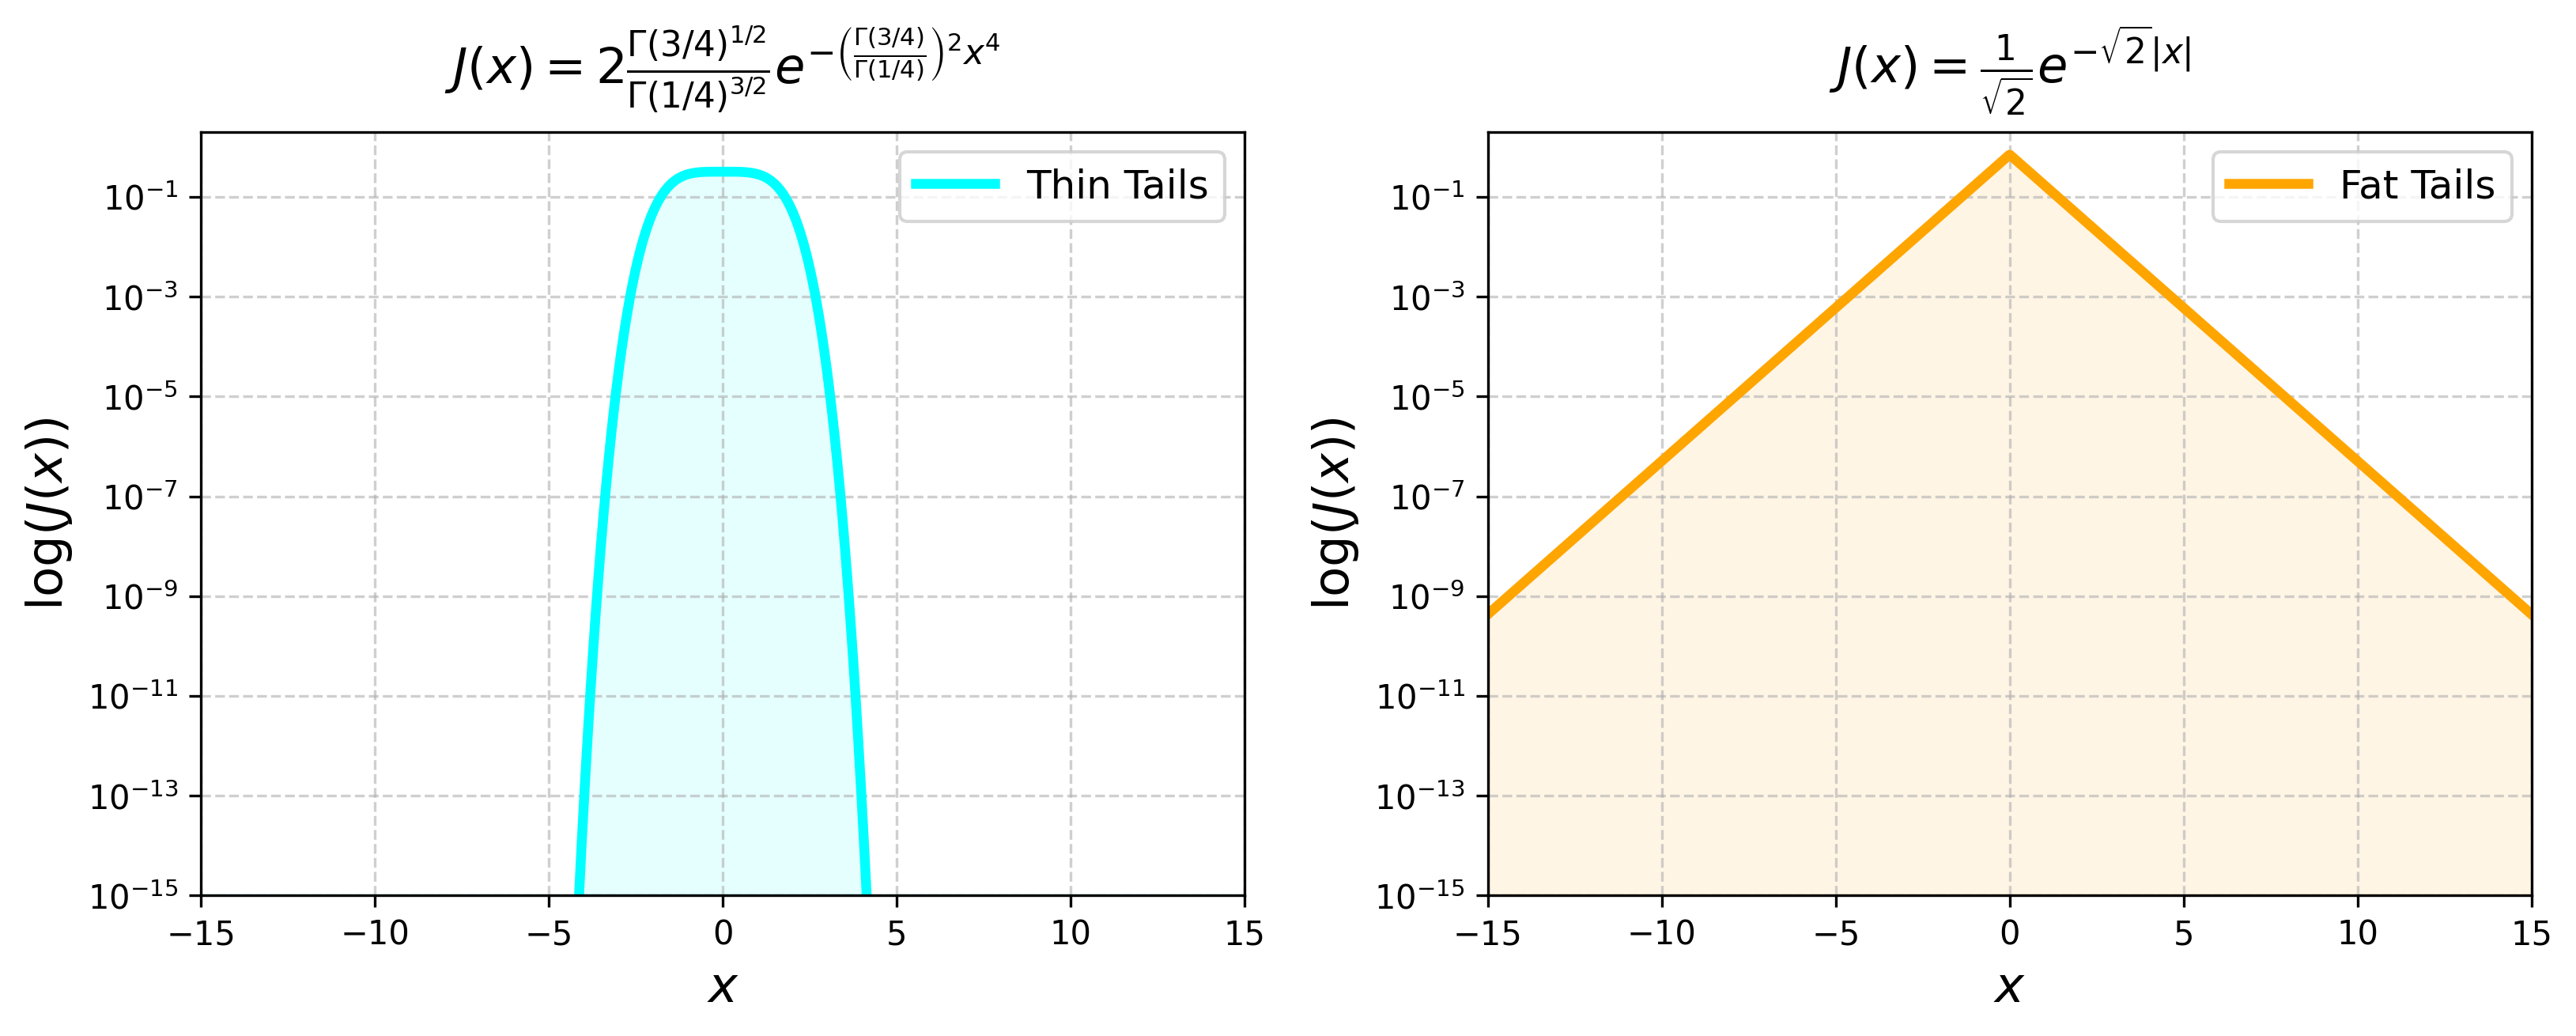
\includegraphics[width=0.9\textwidth]{figures/kernels_1D_log_scale.png}
    \caption{\textcolor{blue}{Visualization of the two-dimensional calibrated dispersal kernels on $\mathbb{R}^2$. Left: the super-Gaussian (thin-tailed) kernel $J_1(x, y) = 2 \left(\frac{\Gamma(3/4)^{1/2}}{\Gamma(1/4)^{3/2}}\right) e^{- \left( \frac{\Gamma(3/4)}{\Gamma(1/4)}\right)^2 x^4}$ displaying a flatter core and rapidly decaying tails. Right: the isotropic sub-Gaussian (fat-tailed) kernel $J_2(x, y) = \frac{1}{\sqrt{2}} e^{-\sqrt{2}|x|}$ characterized by a sharp central peak and extensive tails. Both kernels are normalized to unit volume and calibrated to unit variance over $\mathbb{R}^2$.}}
    \label{fig:dispersal_kernels_1d}
\end{figure}
We shall compare our results to the classical reaction-diffusion system. In order to do that properly, we examine the Taylor expansion of the dispersal operator $\mathcal{L}$ with given kernel $J$:
\begin{equation}
    \label{eq:dispersal_op_taylor_expansion}
    \mathcal{L} v = \frac{1}{2}\left(\int_{\mathbb{R}} J(z)z^2dz\right) \Delta v + \text{h.o.t.}
\end{equation}
With our choice of the kernels $J_1, J_2$ we have that their variances are equal and satisfy the equation
\begin{equation}
    \label{eq:experiment_kernels_equal_variance}
    \int_{\mathbb{R}} J_1(z)z^2 dz = \int_{\mathbb{R}} J_2(z)z^2 dz = 1.
\end{equation}
Consequently, we use the local counterpart of the non-local model \eqref{eq:u}--\eqref{eq:v_init} to examine the effect of the higher-order terms (h.o.t.), given by
\begin{numcases}{}
    v_t = \frac{d_v}{2} \Delta v + v^2 w - B v & \hspace{2mm} $(x, t) \in \Omega \times [0, T],$ \label{eq:local_u} \\
    w_t = d_w\Delta w - v^2w - w + A & \hspace{2mm} $(x, t) \in \Omega \times [0, T],$ \label{eq:local_v} \\
    v = 0 & \hspace{2mm} $(x,t) \in \partial\Omega \times [0,T], $ \label{eq:local_u_bound} \\
    w = 0 & \hspace{2mm} $(x,t) \in \partial\Omega \times [0,T],$ \label{eq:local_v_bound} \\
    v(0) = v_0 & \hspace{2mm} $x \in \Omega ,$ \label{eq:local_u_init} \\
    w(0) = w_0 & \hspace{2mm} $x \in \Omega\,, $ \label{eq:local_v_init}
\end{numcases}

Now, we are ready to discuss the numerical experiments. We begin with the examination of the impact of the patch half-width $L$ on the stationary solutions.

\begin{expe}
    \label{exp:experiment_critical_patch_size}
    We design a numerical experiment to investigate the existence of a critical patch size for vegetation survival, a concept discussed in our theoretical analysis (see Theorem \ref{thm:critical_patch_size}). The experiment's primary goal is to compare the critical patch size of the classical local (reaction-diffusion) model against two distinct non-local models. These non-local models employ dispersal kernels with ``thin tails'' (super-Gaussian) and ``fat tails'' (sub-Gaussian), respectively. Crucially, both non-local kernels are calibrated to have the same variance (second moment), ensuring that their leading-order Taylor approximations are equivalent to the same Laplacian operator. This setup allows us to directly isolate and observe the influence of higher-order terms, which represent the shape of the dispersal kernel, on population persistence.
    
    The simulation framework is configured as follows:
    \begin{itemize}
        \item By Proposition \ref{prp:ExistenceOfConstantSSKineticSystem}, we assume that $A > 2B$ to guarantee the existence of non-zero, spatially uniform vegetation and water solutions $(v_*, w_*)$ of the system \eqref{EQ:ConstantSteadyStates}. In particular, we take mortality $B = 0.45$ and rainfall $A = 1.8$. For this choice of parameters we get that $(v_{*, 3}, w_{*, 3})$ satisfies (A3).
        \item We consider fixed dispersal rate $d_v = 2.0$ and diffusion rate $d_w = 0.1$.
        \item We choose the range of patch half-widths $L \in [10^{0}, 10^2]$. We split this interval into $50$ points equally distributed along the logarithmic scale.
    \end{itemize}
    For each value of $L$, we find the stationary solution for all three models by simulating the system's dynamics. The simulation is performed using a forward Euler time-stepping scheme with a time step of $h_t = 10^{-4}$. The system is considered to have reached a steady state when the $\ell^2$-norm of the difference between consecutive time steps falls below a tolerance of $\epsilon_{\text{tol}} = 10^{-5}$. To encourage convergence to non-trivial solutions, the initial condition for each simulation is given by the spatially uniform steady state $(v_{*,3}, w_{*,3})$, which is then perturbed by a small cosine profile. The spatial domain is discretized using a number of equidistant nodes $N$ that increases proportionally with $L$ to maintain adequate numerical resolution across all scales.

    To quantify the results, we record the average biomass density of the final stationary solution for each $L$. The critical patch size, $L_{\text{crit}}$, is then numerically determined for each model as the largest patch half-width for which the average biomass falls below a small threshold of $0.1$.
\end{expe}
We present the results of our numerical simulations in the figure below.
\begin{figure}[H]
    \centering
    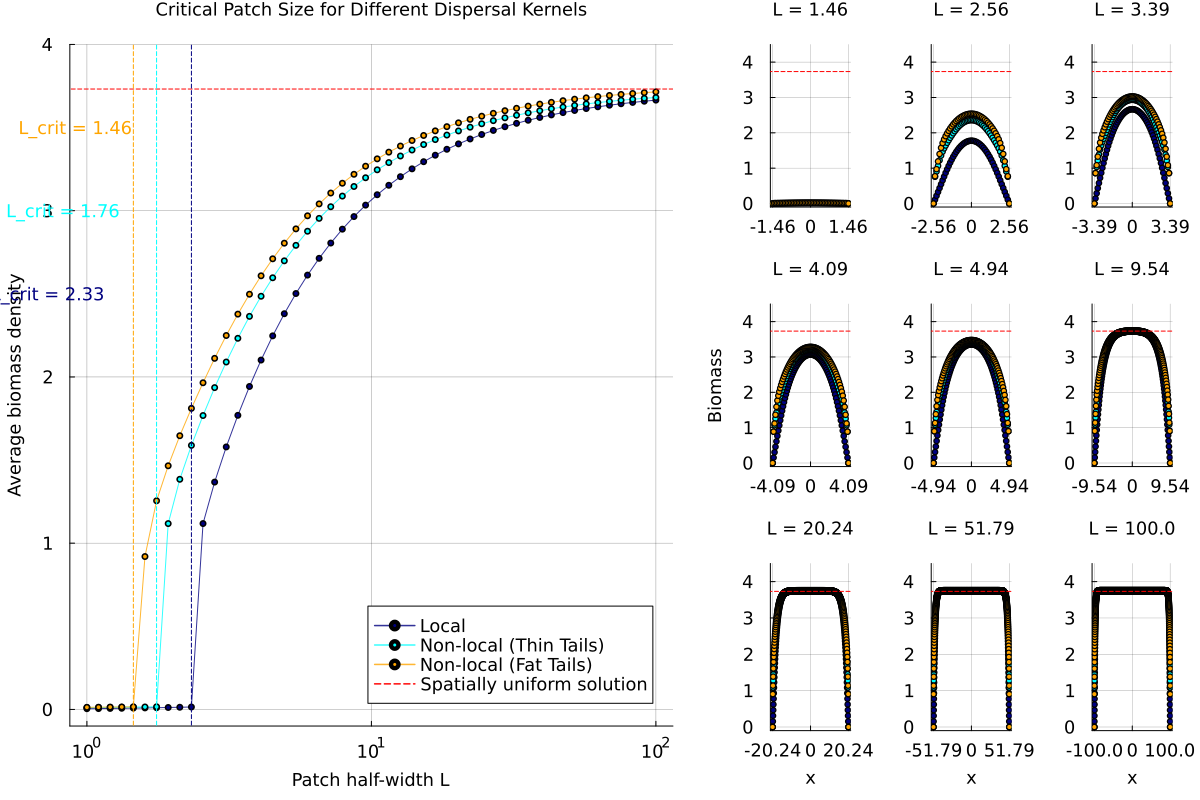
\includegraphics[width=\textwidth]{figures/critical_patch_size_dv2_dw01.png}
    \caption{In the left panel, we show the spatially uniform steady-state solution $v_{*,3}$ (red dashed line), the average stationary biomass in the non-local models with thin and fat tails (cyan and orange, respectively) and in the local model (blue) as a function of the patch half-width $L$. We also present the corresponding, numerically estimated critical patch sizes (dashed vertical lines). In the right panel, we present a gallery of stationary biomass density profiles (orange, cyan and blue dots) for different patch half-widths $L$, corresponding to the results shown in the left panel. The parameters used here are described in Experiment \ref{exp:experiment_critical_patch_size}.}
    \label{fig:critical_patch_size}
\end{figure}
\begin{con}
As shown in the left panel of Figure \ref{fig:critical_patch_size}, all three models—local, non-local with thin tails, and non-local with fat tails—exhibit the same qualitative behavior for large domains. Specifically, their respective stationary solutions converge to the spatially uniform steady state $v_{*, 3}$ as the patch half-width $L$ increases and boundary effects become negligible. This agrees with our existence and stability results contained in Theorems \ref{thm:Stationary-Solutions-Existence} and \ref{thm:Stationary-Solutions-Stability}.
\end{con}

\begin{con}
The left panel of Figure \ref{fig:critical_patch_size} reveals that, while all models eventually collapse to the desert state, the critical patch size required for survival is different for each. The model with the fat-tailed (sub-Gaussian) kernel is the most resilient, exhibiting the smallest critical patch size ($L_{\text{crit}} \approx 1.46$). This is followed by the thin-tailed (super-Gaussian) kernel ($L_{\text{crit}} \approx 1.76$), while the local model is the least resilient, requiring the largest habitat for survival ($L_{\text{crit}} \approx 2.33$). Since all non-local kernels were calibrated to have the same variance, this ordering is directly attributable to the influence of higher-order moments. This provides evidence that long-range dispersal events, which are more frequent in kernels with a larger fourth moment (kurtosis), significantly enhance the ability of vegetation to persist in smaller, fragmented habitats.
\end{con}

\begin{con}
The right panel of Figure \ref{fig:critical_patch_size} shows a difference in the solution profiles at the domain boundary. The local model's solution, governed by diffusion, is continuous and smoothly approaches zero. In contrast, both non-local models exhibit a sharp drop-off at the boundary. This is a direct consequence of Theorem \ref{thm:Stationary-Solutions-Existence}, namely equation \eqref{eq:f_ball_to_ball_radius} defining the distance $R_*$ between the constant value $v_{*, 3}$ and the stationary solution $V$. Note that for small diffusion and dispersal rates $d_v, d_w$ it is true that $R_* < v_{*, 3}$, directly implying discontinuity at the boundary.
\end{con}

\begin{expe}
    We propose an experiment in which we investigate the existence of a critical level of concentration of the vegetation as in Theorem \ref{thm:Exinction-Of-Vegetation}. We proceed by computing the bifurcation diagram for the local and non-local Klausmeier model. Having that, we will check if the branches are bounded from below by $\sim\frac{B}{A}$. In the regime of decreasing rainfall $A$ the stationary vegetation $V$ obtained by Theorems \ref{thm:Stationary-Solutions-Existence} and \ref{thm:Stationary-Solutions-Stability} ceases to exist once $A = 2B$. We also want to validate whether there exists a regime of parameters $d_v, d_w$ such that inhomogeneous solutions emerge. We assume the following framework of the experiment:
    \begin{itemize}
        \item We vary the rainfall $A \in [0.1, 3.0]$ with fixed mortality $B = 0.45$.
        \item We consider the dispersal rate $d_v = 2.0$ and diffusion rate $d_w \in \{0.1, 80.0\}$.
        \item We take the patch half-width $L = 25$.
    \end{itemize}
    The bifurcation diagrams were generated using the Julia package \texttt{BifurcationKit.jl}. The numerical method relies on a Pseudo-Arclength Continuation (PALC) algorithm to trace solution branches. For the spatial discretization, the domain $\Omega = (-L, L)$ is discretized using $N = \lfloor 3L \rfloor$ equidistant nodes. The Laplacian operator $\Delta$ is approximated using a standard second-order centered finite difference scheme, and the non-local integral operator $\mathcal{L}$ is approximated using the composite trapezoidal rule. The convergence tolerance $\epsilon$ for the underlying Newton solver was set to $\epsilon = 10^{-10}$.

    The continuation process was initiated from the parameter value $A = 3.0$. The initial guess was constructed from the spatially homogeneous steady state $(v_0, w_0) = (v_{*, 3}, w_{*, 3})$, as given by Proposition \ref{prp:ExistenceOfConstantSSKineticSystem}, with a small cosine-shaped spatial perturbation applied to encourage convergence to non-uniform solution branches.
\end{expe}

We present the results of numerical simulations done in the regime of slow diffusion, e.g.\ with $d_w = 0.1$.

\begin{figure}[H]
    \centering
    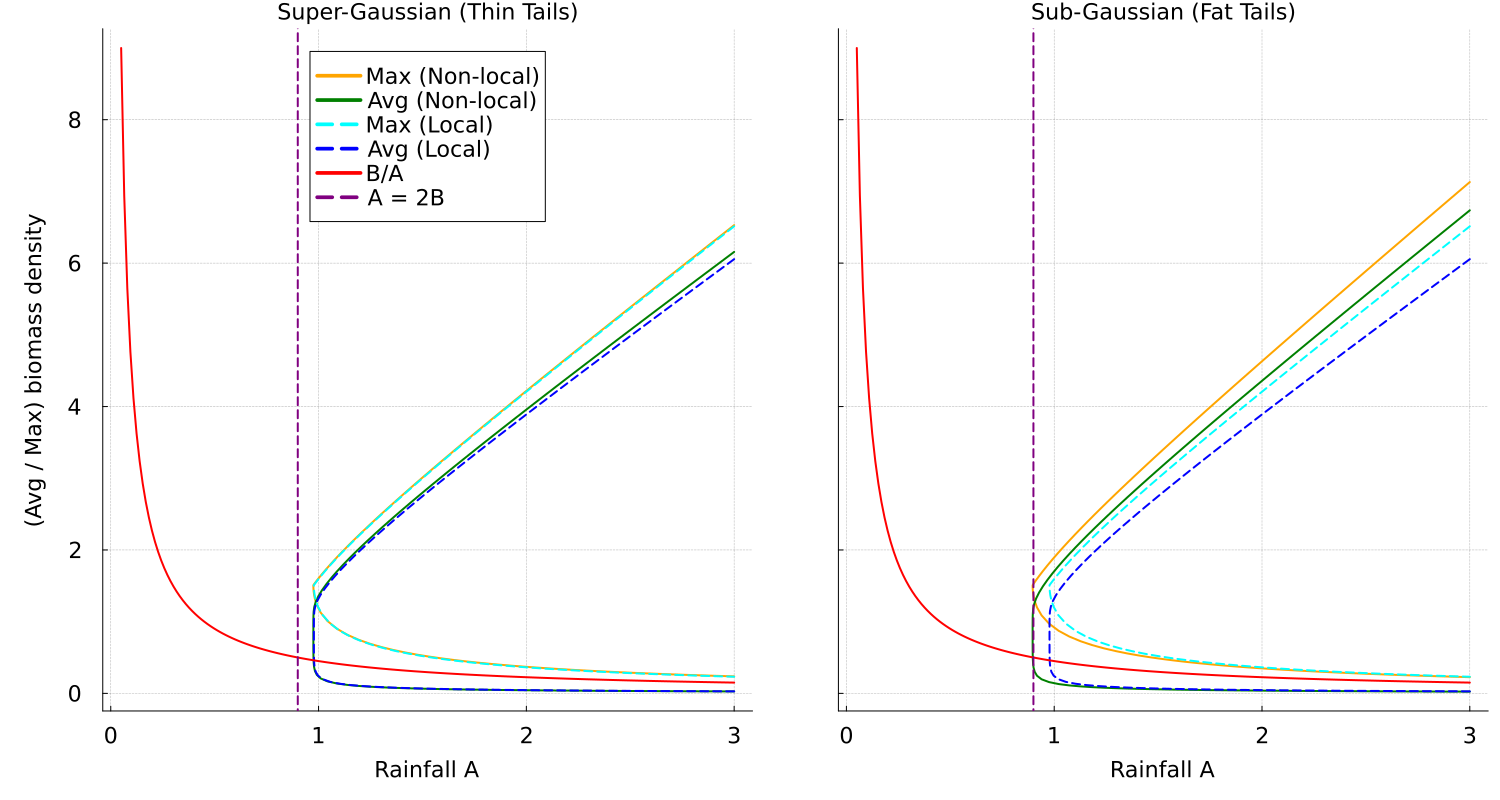
\includegraphics[width=\textwidth]{figures/bifurcation_diagram_dv2_dw01.png}
    \caption{Comparison of bifurcation diagrams for the non-local models using a super-Gaussian (thin tails) and a sub-Gaussian (fat tails) dispersal kernel, both shown against the standard local model. Solid orange and green lines represent the maximum and average biomass for the non-local models, while dashed cyan and blue lines show the same for the local model. We mark the critical biomass threshold (red line, $\sim B/A$) and the critical rainfall for the kinetic system (purple line, $A=2B$). Here $d_v = 2.0, d_w = 0.1, B = 0.45$.}
    \label{fig:bifurcation_diagram_slow}
\end{figure}

\begin{con}
    The results shown in Figure \ref{fig:bifurcation_diagram_slow} align with our theoretical results from Theorem \ref{thm:Exinction-Of-Vegetation}. In particular, every stationary solution has the maximal value bounded from below by the value $\sim B/A$.
\end{con}

\begin{con}
    Our simulation confirms the statement of Theorems \ref{thm:Stationary-Solutions-Existence}, \ref{thm:Stationary-Solutions-Stability}, namely the existence of a stable, spatially perturbed steady state up to the point when the rainfall $A$ approaches the value $A = 2B$. When $A < 2B$, the spatially uniform solutions $(v_{*, 3}, w_{*, 3})$ cease to exist and the vegetation goes extinct.
\end{con}

Finally, we show the results of numerical simulations done in the regime of fast diffusion, e.g.\ with $d_w = 80.0$.

\begin{figure}[H]
    \centering
    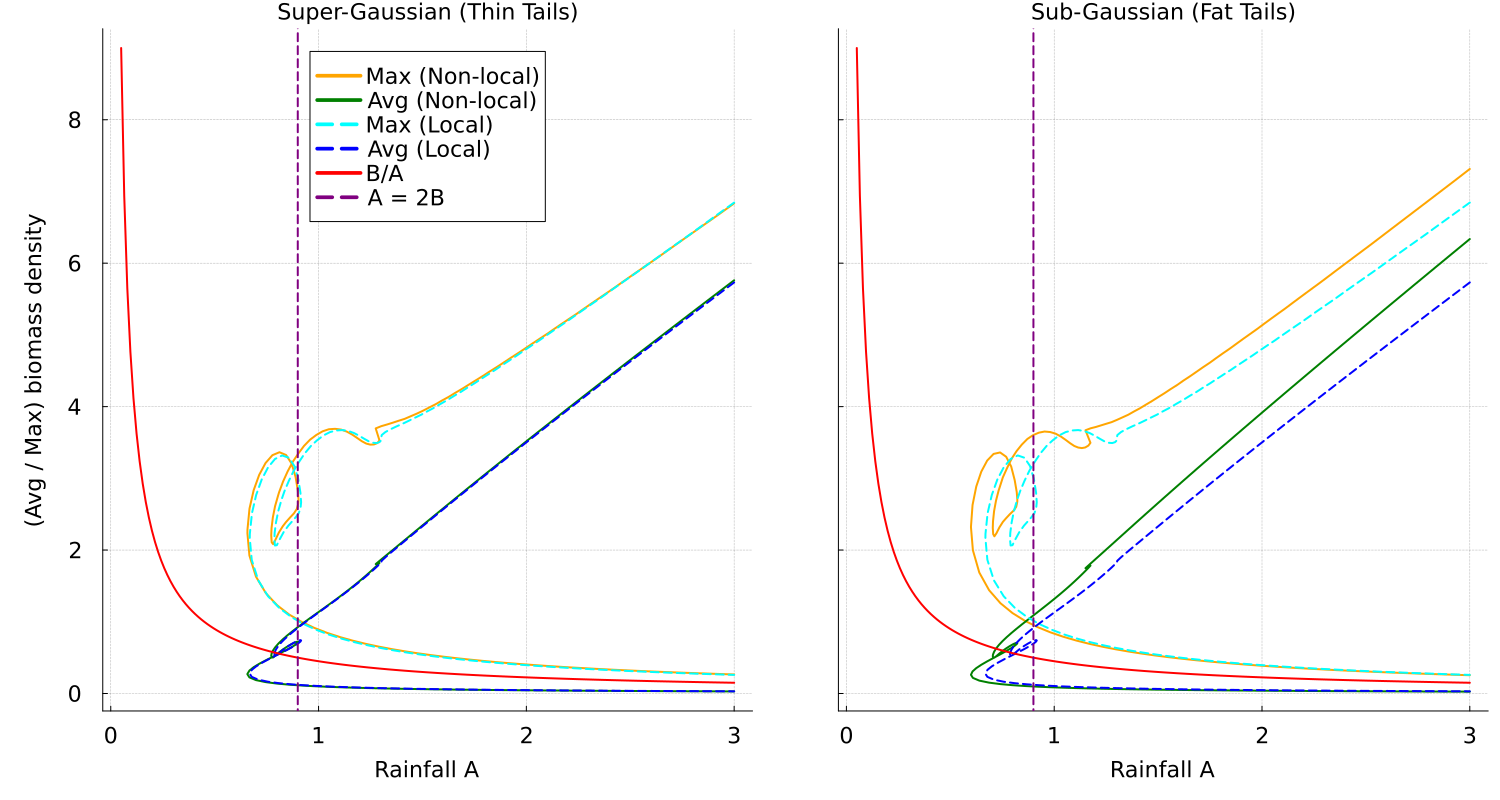
\includegraphics[width=\textwidth]{figures/bifurcation_diagram_dv2_dw80.png}
    \caption{Comparison of bifurcation diagrams for the non-local models using a super-Gaussian (thin tails) and a sub-Gaussian (fat tails) dispersal kernel, both shown against the standard local model. Solid orange and green lines represent the maximum and average biomass for the non-local models, while dashed cyan and blue lines show the same for the local model. We mark the critical biomass threshold (red line, $\sim B/A$) and the critical rainfall for the kinetic system (purple line, $A=2B$). Here $d_v = 2.0, d_w = 80.0, B = 0.45$.}
    \label{fig:bifurcation_diagram_fast}
\end{figure}

\begin{con}
    A comparison of the bifurcation diagrams in Figure \ref{fig:bifurcation_diagram_fast} reveals the impact of the dispersal kernel's shape on the system's dynamics. While both the super-Gaussian (thin tails) and sub-Gaussian (fat tails) models support complex, looping solution branches, the sub-Gaussian kernel yields the existence of non-deserted solutions over a wider range of the rainfall parameter $A$. The oscillatory behavior suggests a cascade of secondary bifurcations. Notably, in both non-local scenarios, patterned solutions emerge for rainfall levels below the kinetic system's threshold ($A < 2B$).
\end{con}

\begin{con}
    Across all models presented in Figures \ref{fig:bifurcation_diagram_slow} and \ref{fig:bifurcation_diagram_fast}, the curve $\sim B/A$ serves as a sharp lower bound for the biomass of all non-trivial stationary solutions. This provides robust numerical validation for the vegetation extinction threshold predicted by Theorem \ref{thm:Exinction-Of-Vegetation}, confirming its applicability to both local and a range of non-local dispersal strategies.
\end{con}

For the sake of exposition we provide the spatial visualization of patterns obtained in Figure \ref{fig:bifurcation_diagram_fast}.

\begin{figure}[H]
    \centering
    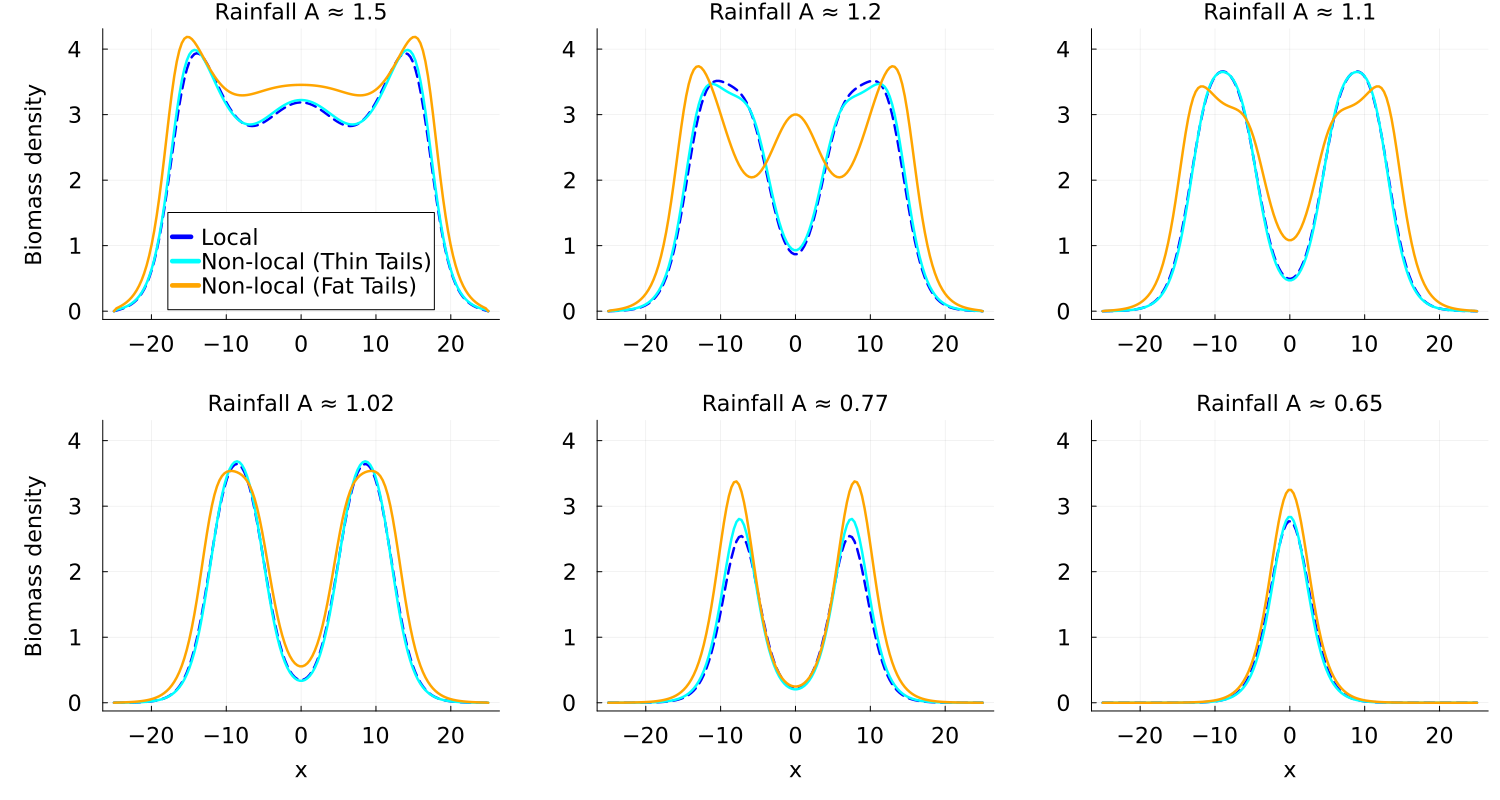
\includegraphics[width=\textwidth]{figures/bifurcation_profiles_dv2_dw80.png}
    \caption{A gallery of stationary biomass densities for non-local and local models (green and blue dashed lines respectively). We selected several points from the upper branch of the rightmost bifurcation diagram in Figure \ref{fig:bifurcation_diagram_fast}. Here $d_v =2.0, d_w = 80.0, B = 0.45, L=25$.}
    \label{fig:bifurcation_profiles_fast}
\end{figure}

\begin{con}
    The bifurcation diagram for the fat-tailed kernel $J_2$ with patch half-width $L=25$ shown in Figure \ref{fig:bifurcation_diagram_fast} gives very similar loopy structures in both models. However, the vegetation profiles corresponding to this diagram, presented in Figure \ref{fig:bifurcation_profiles_fast}, do not always share the same geometry with respect to the local / non-local model, particularly for $A = 1.2$. It is also worth noting that, due to the high diffusion regime, the characteristic sharp drop-off at the boundary has disappeared.
\end{con}

\subsection{Two-dimensional simulations}

Extending the numerical bifurcation analysis to two-dimensional spatial domains poses significant computational challenges. Standard continuation packages, such as \texttt{BifurcationKit.jl} used in the one-dimensional case, often struggle with the dense Jacobian matrices arising from non-local integral operators on 2D grids, frequently leading to memory exhaustion or divergence of the underlying Newton solver. To overcome this limitation and complement our 1D findings, we implemented a custom numerical continuation routine tailored for the two-dimensional Klausmeier model.

This custom solver traces the stationary solution branches by sequentially decreasing the rainfall parameter $A$. At each parameter step, the stationary state is found by solving the implicit Euler discretization of equations \eqref{eq:u}--\eqref{eq:v_init} until a steady state is reached. To ensure numerical stability and handle the dense non-local terms efficiently without assembling the full Jacobian, we employ an iterative Gauss--Seidel method. While this approach allows us to successfully trace the stable branches of the bifurcation diagram and obtain 2D spatial profiles, it is important to note that, unlike pseudo-arclength continuation, this simple sequential method cannot follow unstable branches or trace the solutions around folds (turning points). Therefore, the 2D results presented here serve as an initial exploration of the spatial morphology in higher dimensions, and a more exhaustive continuation analysis remains an objective for future work.

For demonstrations in the two-dimensional case, we consider the square domain $\Omega = (-L, L) \times (-L, L)$. The two-dimensional super-Gaussian and sub-Gaussian dispersal kernels, calibrated to have a unit variance over $\mathbb{R}^2$, are defined as \textcolor{blue}{(Fig.\,\ref{fig:dispersal_kernels_2d}}):

\begin{equation}
    \label{eq:2dGaussian_PDF}
    J_1(x, y) = \frac{2}{\pi^2} e^{-\frac{1}{\pi} (x^2+y^2)^2}, \quad
    J_2(x, y) = \frac{3}{\pi} e^{-\sqrt{6}\sqrt{x^2+y^2}}, \quad
    (x,y) \in \mathbb{R}^2.
\end{equation}
%\textcolor{blue}{For the sake of the exposition we present visualizations of the two-dimensional dispersal kernels below.}
\begin{figure}[H]
    \centering
    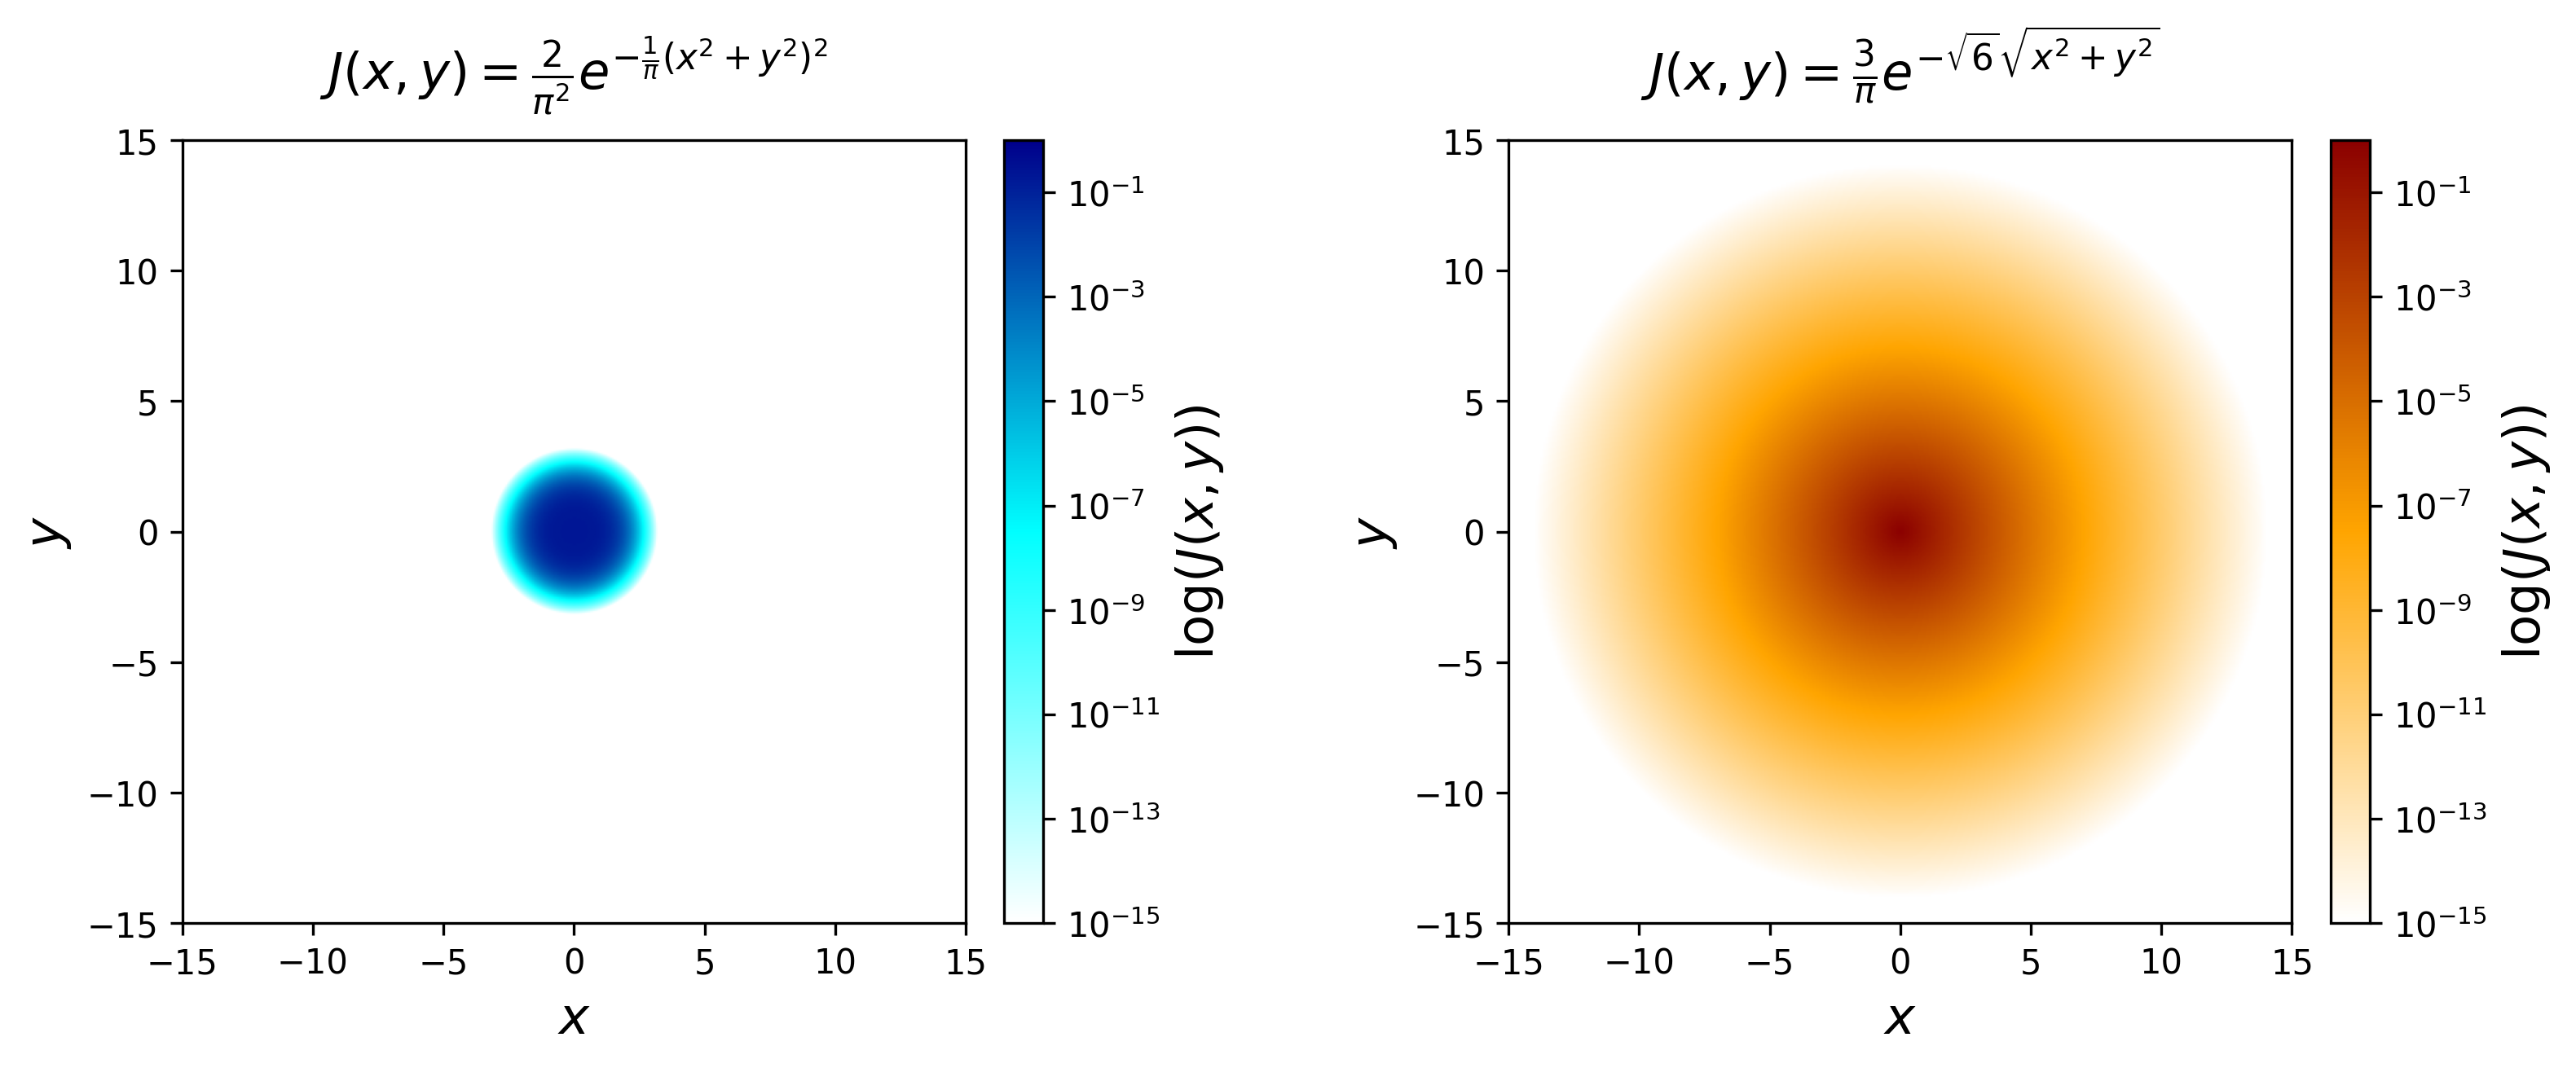
\includegraphics[width=0.9\textwidth]{figures/kernels_2D_log_heatmaps.png}
    \caption{\textcolor{blue}{Visualization of the two-dimensional calibrated dispersal kernels on $\mathbb{R}^2$. Left: the super-Gaussian (thin-tailed) kernel $J_1(x, y) = \frac{2}{\pi^2} e^{-\frac{1}{\pi} (x^2+y^2)^2}$ displaying a flatter core and rapidly decaying tails. Right: the isotropic sub-Gaussian (fat-tailed) kernel $J_2(x, y) = \frac{3}{\pi} e^{-\sqrt{6}\sqrt{x^2+y^2}}$ characterized by a prominent central peak and extensive tails. Both kernels are normalized to unit volume and calibrated to unit variance over $\mathbb{R}^2$.}}
    \label{fig:dispersal_kernels_2d}
\end{figure}
We now describe the specific configuration for exploring the 2D spatial patterns.

\begin{expe}
    We design a numerical experiment to visualize the two-dimensional spatial distribution of biomass and water for the local model and the two non-local models defined by kernels \eqref{eq:2dGaussian_PDF}. The primary goal is to observe the morphological differences in pattern formation induced by the fat-tailed and thin-tailed dispersal strategies in a finite 2D habitat, particularly as environmental conditions become increasingly harsh.
    
    The simulation framework is configured as follows:
    \begin{itemize}
        \item We set the mortality $B = 0.45$, the plant dispersal rate $d_v = 1.0$, and the water diffusion rate $d_w = 10.0$.
        \item The spatial domain is a square with half-width $L = 25.0$. The domain is discretized into a uniform grid of $N \times N$ nodes, with $N = 50$, yielding a system of $2 \times 2500$ variables.
        \item We vary the rainfall parameter $A$ from $A_{\text{max}} = 1.8$ down to $A_{\text{min}} = 0.1$ in $100$ equidistant steps.
        \item At the initial step ($A = 1.8$), the simulation starts from the spatially uniform steady state $(v_{*,3}, w_{*,3})$, perturbed by a small amount of random noise to trigger pattern formation. Dirichlet boundary conditions ($v=0, w=0$) are strictly enforced at the boundaries of the square domain at all times.
        \item For each subsequent value of $A$, the converged stationary solution from the previous step is used as the initial guess for the Gauss--Seidel solver. The system is evolved with a time step of $h_t = 0.01$ until the sum of the $\ell^2$-norms of the differences in $v$ and $w$ between consecutive iterations falls below $\epsilon_{\text{tol}} = 10^{-3}$, or until a maximum of $100,000$ iterations is reached.
    \end{itemize}
    We record the stationary 2D profiles of biomass density $v(x,y)$ and water density $w(x,y)$ along the parameter branch. We then select several representative values of rainfall $A$ to compile a gallery comparing the spatial patterns generated by the local, thin-tailed, and fat-tailed models.
\end{expe}

Below, we present the 2D gallery of spatial patterns we were able to produce using our iterative Gauss-Seidel approach. We start with the local reaction-diffusion model.

\begin{figure}[H]
    \centering
    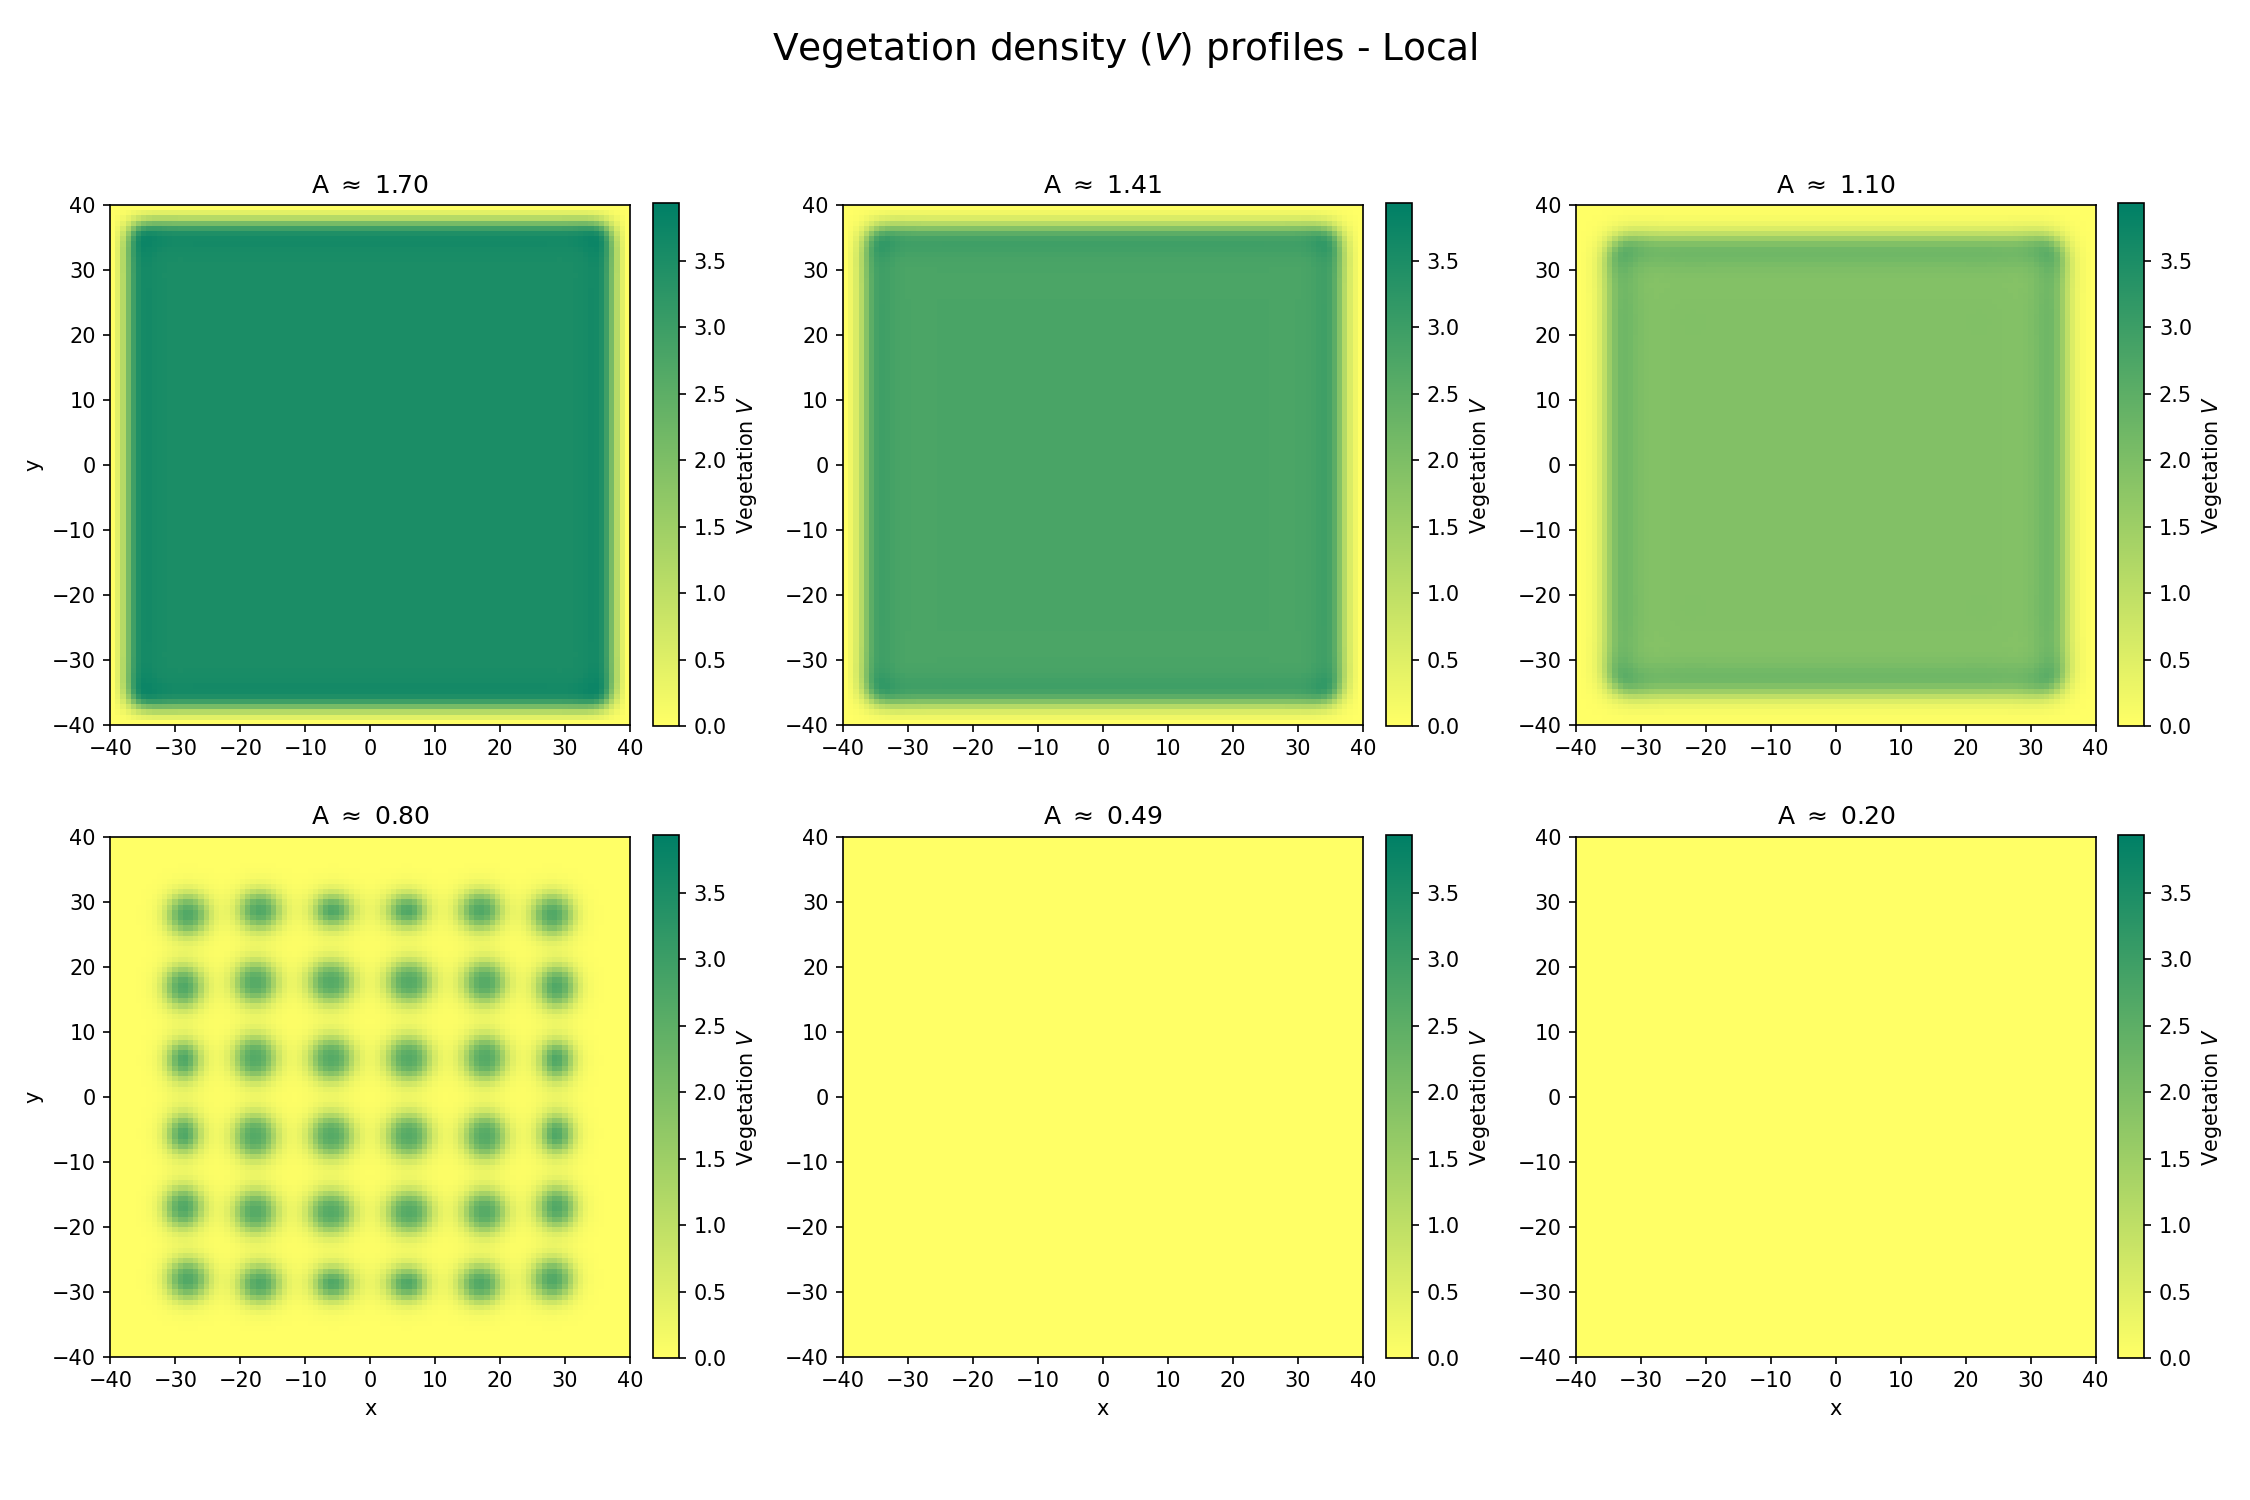
\includegraphics[width=\textwidth]{figures/gallery_V_kernel_local_B_0.45_L_40.0_dv_1.0_dw_10.0.png}
    \caption{A gallery of two-dimensional stationary vegetation biomass density ($V$) profiles for the classical local reaction-diffusion model at various precipitation levels $A$. Here $d_v = 1.0, d_w = 10.0, B = 0.45, L = 40.0$.}
    \label{fig:gallery_local}
\end{figure}

\begin{con}
    The two-dimensional local model (Figure \ref{fig:gallery_local}) exhibits a classic pattern formation sequence. At high precipitation levels ($A \ge 1.10$), the biomass is uniformly distributed in the interior and smoothly decays to zero near the hostile boundaries. As rainfall decreases ($A \approx 0.80$), the uniform state breaks down into a regular array of isolated vegetation spots that gradually fade at the edges of the domain. Further reduction in rainfall leads to a complete ecosystem collapse, with the domain turning into a bare desert already at $A \approx 0.49$.
\end{con}

Now, we move to the non-local model with a thin-tailed dispersal kernel.

\begin{figure}[H]
    \centering
    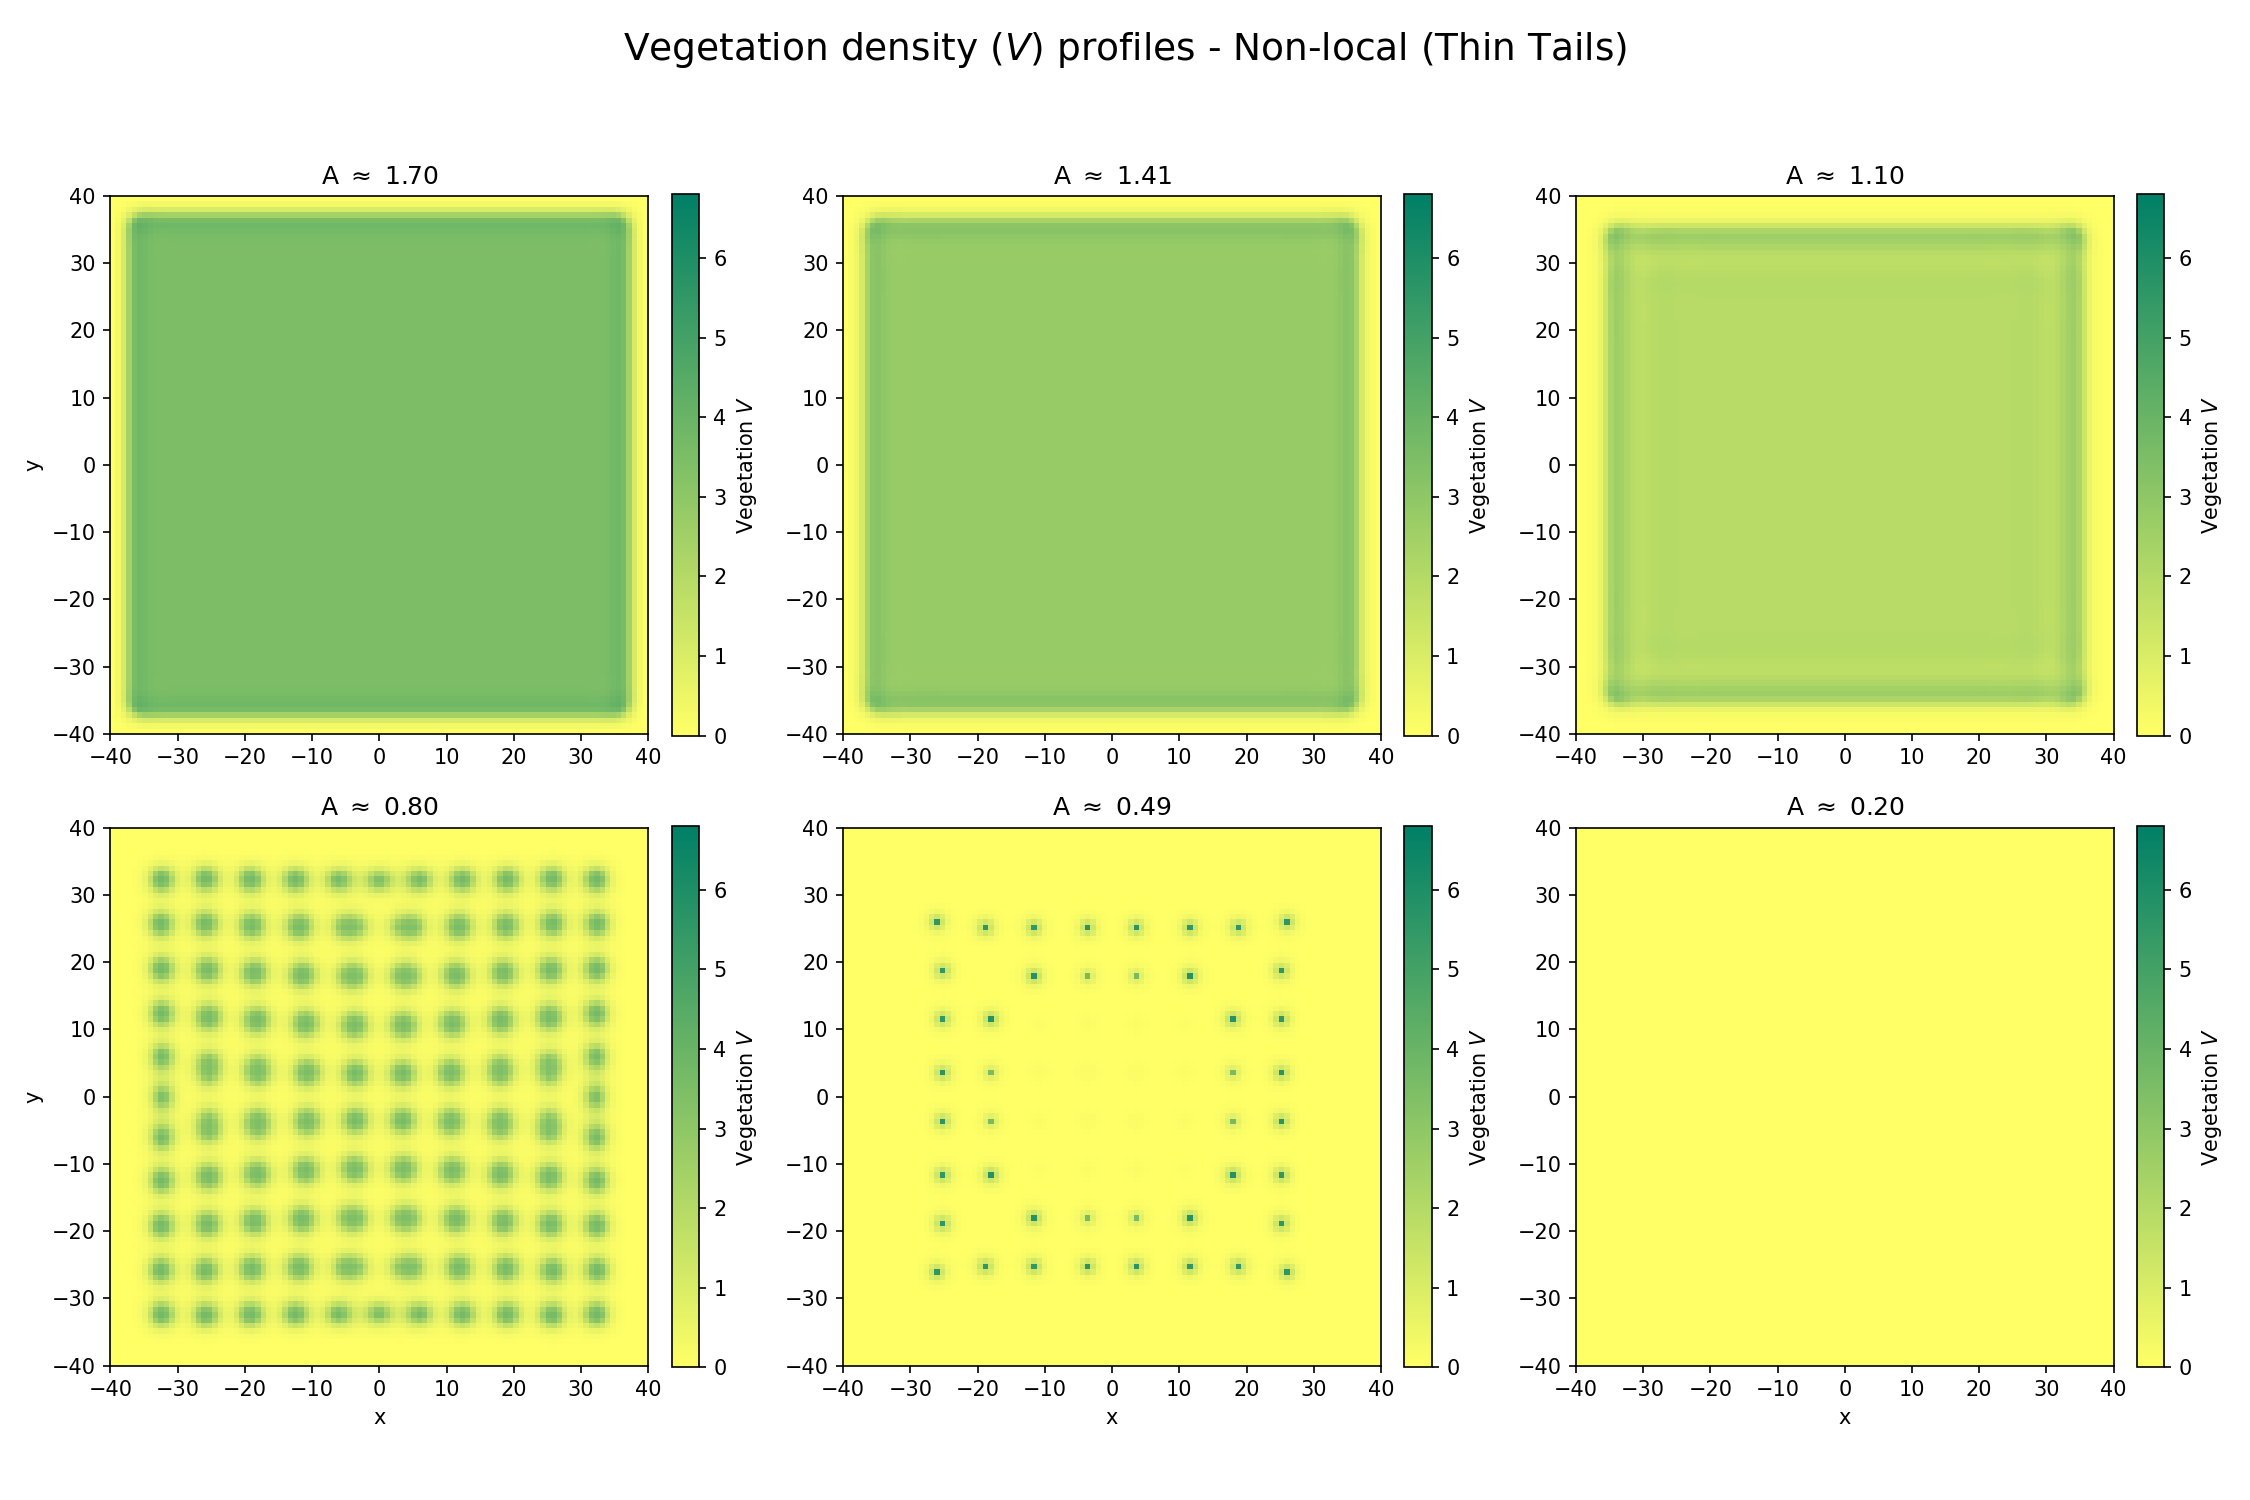
\includegraphics[width=\textwidth]{figures/gallery_V_kernel_thin_tails_B_0.45_L_40.0_dv_1.0_dw_10.0.png}
    \caption{A gallery of two-dimensional stationary vegetation biomass density ($V$) profiles for the non-local model with a super-Gaussian (thin-tailed) dispersal kernel at various precipitation levels $A$. Here $d_v = 1.0, d_w = 10.0, B = 0.45, L = 40.0$.}
    \label{fig:gallery_thin}
\end{figure}

\begin{con}
    Introducing non-local dispersal with thin tails (Figure \ref{fig:gallery_thin}) preserves the general transition from uniform cover to spotted patterns, but introduces notable differences compared to the local model. Most importantly, the vegetation exhibits enhanced resilience, maintaining a sparse array of spots at $A \approx 0.49$, an aridity regime where the local model has already collapsed.
\end{con}

And finally, we present the non-local model with a fat-tailed dispersal kernel.

\begin{figure}[H]
    \centering
    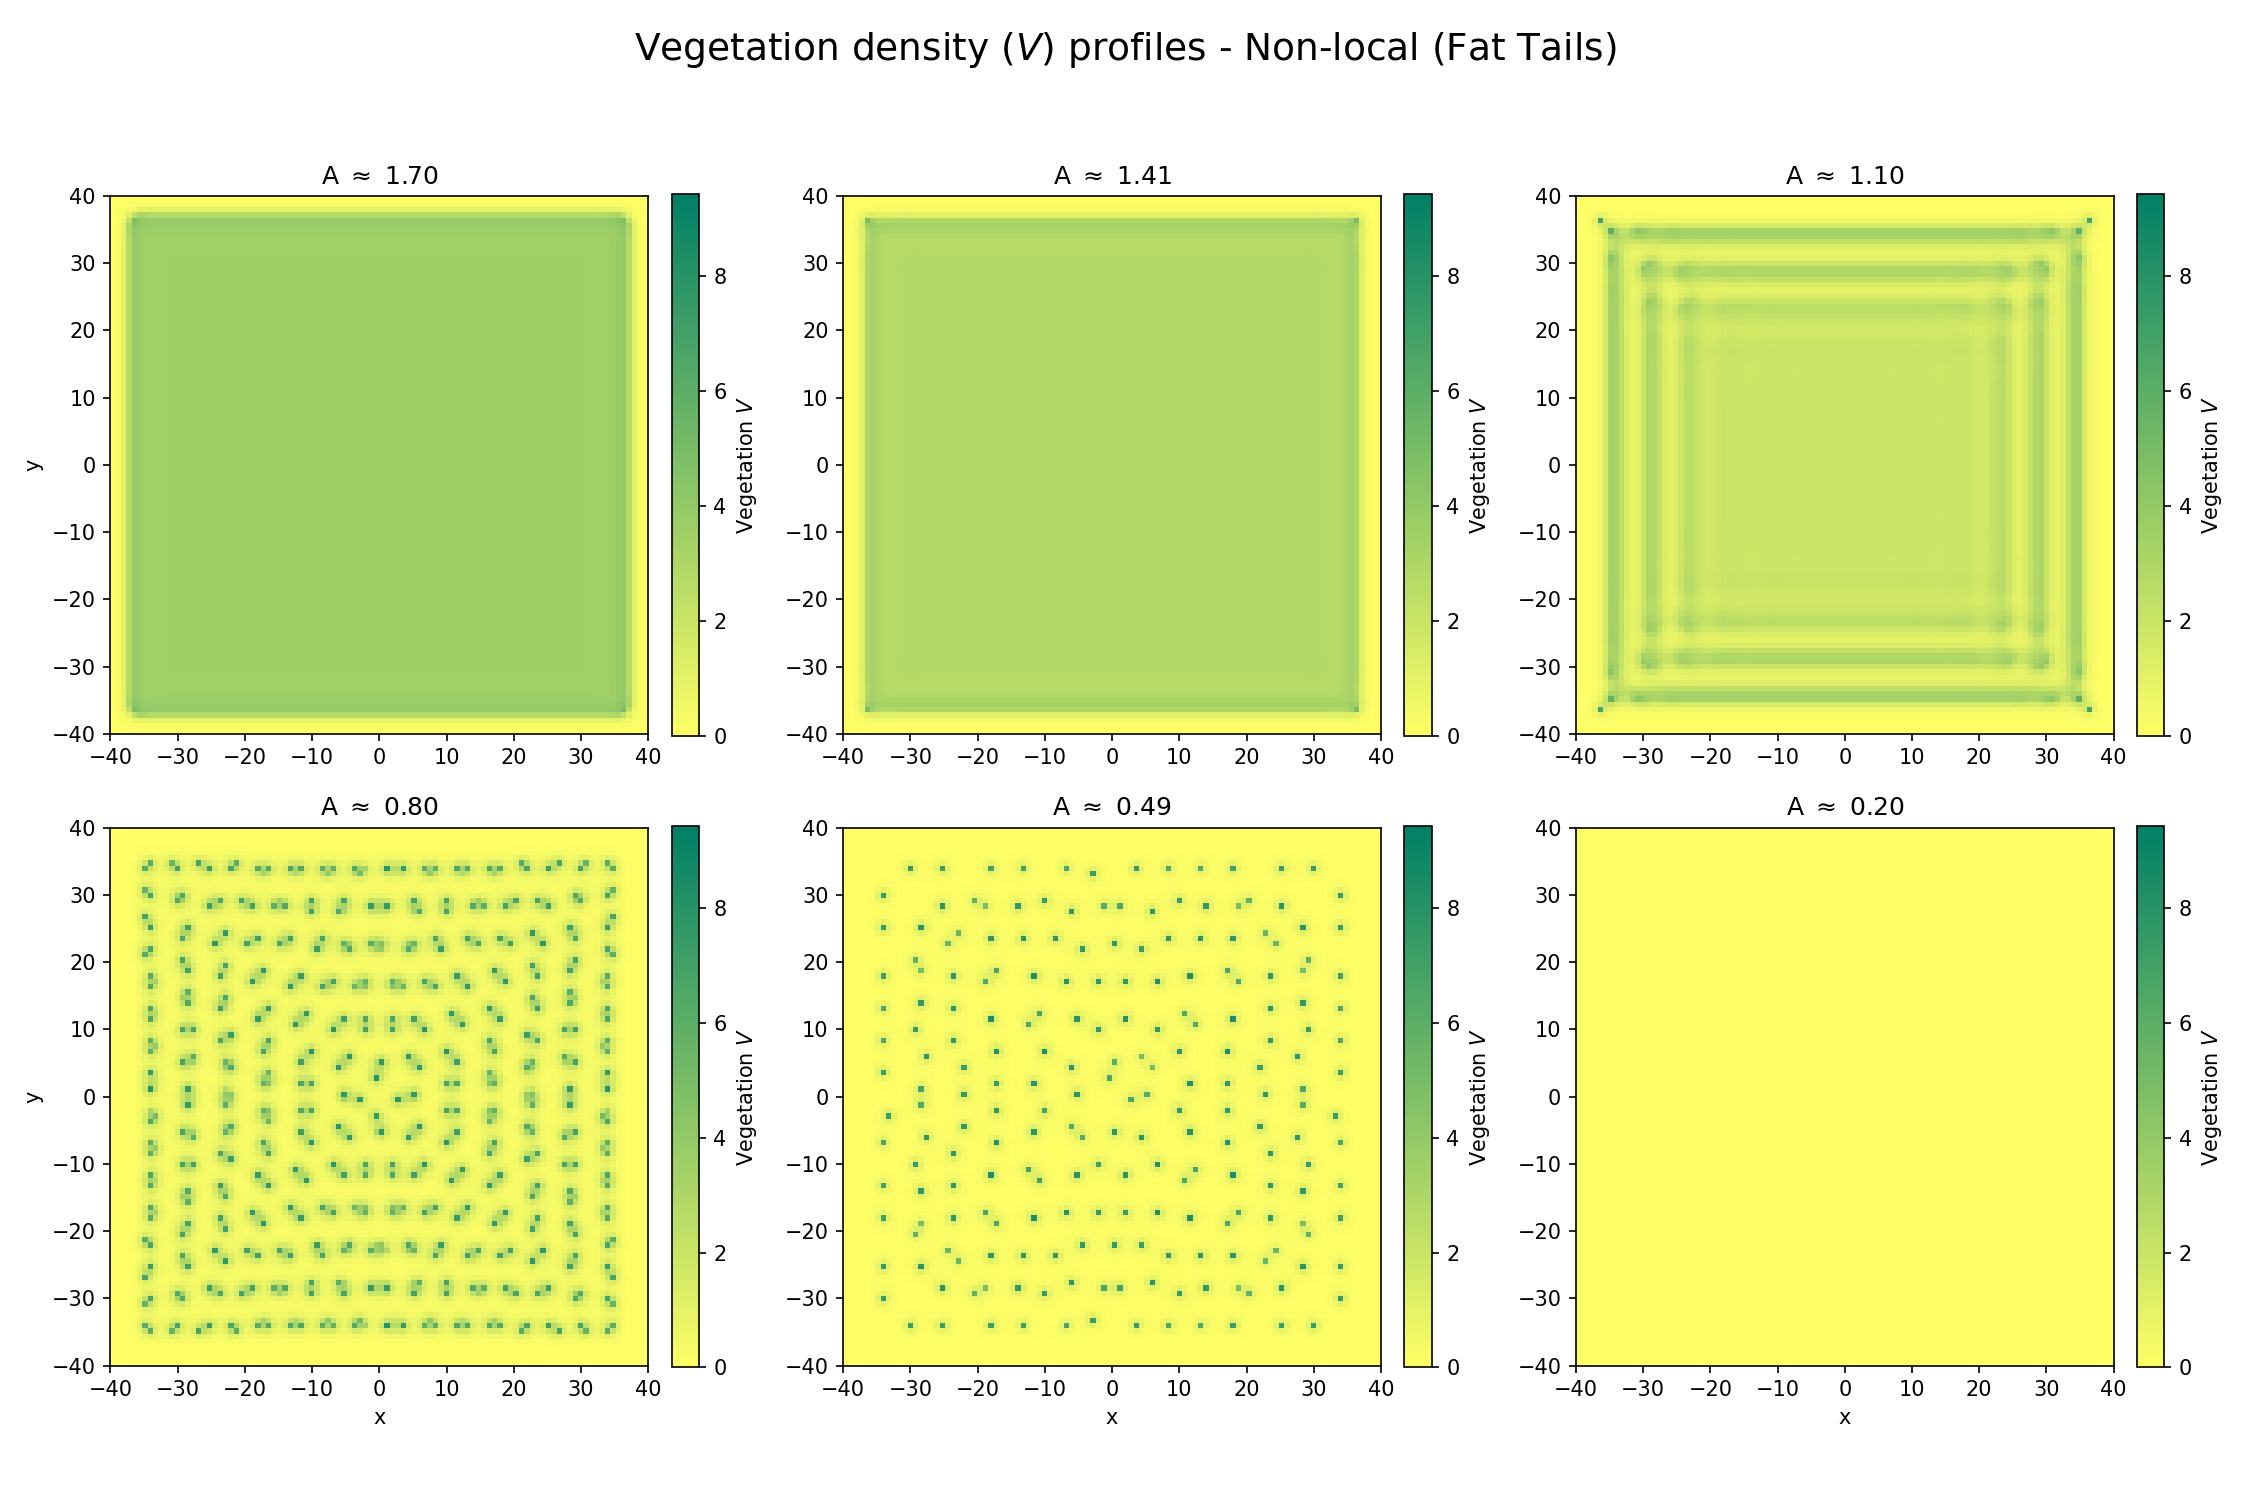
\includegraphics[width=\textwidth]{figures/gallery_V_kernel_fat_tails_B_0.45_L_40.0_dv_1.0_dw_10.0.png}
    \caption{A gallery of two-dimensional stationary vegetation biomass density ($V$) profiles for the non-local model with a sub-Gaussian (fat-tailed) dispersal kernel at various precipitation levels $A$. Here $d_v = 1.0, d_w = 10.0, B = 0.45, L = 40.0$.}
    \label{fig:gallery_fat}
\end{figure}

\begin{con}
    The impact of higher-order moments becomes most striking in the non-local model with a fat-tailed dispersal kernel (Figure \ref{fig:gallery_fat}). While it shares the enhanced resilience observed in the thin-tailed model (similarly surviving at $A \approx 0.49$), its spatial morphology is fundamentally different. A highly pronounced, continuous boundary ridge of high vegetation density forms along the edges of the habitat for a wide range of precipitation levels. This strongly contrasts with the smooth decay of the local model and the isolated boundary spots of the super-Gaussian model. This prominent boundary aggregation provides a clear 2D visualization of the sharp drop-off phenomenon predicted by our one-dimensional theoretical and numerical analyses, confirming that long-range dispersal induces profound structural changes in fragmented ecosystems.
\end{con}

\textcolor{blue}{
\begin{con}
    The complex, grid-like spot patterns observed for $A \approx 0.80$ and $A \approx 0.49$ in the fat-tailed model (Figure 7) are a direct manifestation of the self-replication phenomenon. As documented in previous studies on vegetation dynamics and localized structures \cite{BordeuEtAl2015, BordeuEtAl2016, TlidiEtAl2018}, when precipitation decreases, the interplay between short-range plant facilitation and strong non-local competition for water drives a curvature (or ring) instability. As a localized vegetation patch or a continuous boundary ridge grows, it severely depletes the water resources in its center. Consequently, the core of the structure experiences extreme hydric stress and dies off, forcing the patch to elongate and split into new, distinct spots. This continuous self-replication mechanism enables the vegetation to actively colonize empty territories and maximize spatial water use efficiency. Ecologically, this dynamic spatial reshaping acts as an anti-desertification strategy; it allows the ecosystem to maintain a higher total biomass and prevent a shift into a desert state.
\end{con}
}

\subsection{Discussion and ecological implications}

In this work, we established the mathematical framework for a generalized, non-dimensionalized Klausmeier model incorporating non-local plant dispersal on finite, flat domains. We proved the local-in-time well-posedness of the system \eqref{eq:u}--\eqref{eq:v_init} and the existence of an invariant region guaranteeing non-negative, bounded solutions. Utilizing a fixed-point argument, we constructed non-trivial stationary solutions bifurcating from the uniform steady states, as formalized in Theorem \ref{thm:Stationary-Solutions-Existence}. Furthermore, we derived precise criteria governing the long-time asymptotic behavior of these solutions. Theorem \ref{thm:Exinction-Of-Vegetation} establishes sufficient conditions for inevitable convergence to the trivial desert state based on the initial biomass concentration, while Theorem \ref{thm:Stationary-Solutions-Stability} dictates the parameter regime, specifically requiring sufficiently small transport rates $d_v$ and $d_w$, under which the non-trivial spatially structured solutions are linearly exponentially stable.

These analytical foundations were subsequently complemented by extensive numerical experiments. By calibrating the non-local dispersal kernels to share the same variance as the classical Laplacian operator, we isolated the impact of higher-order moments on the system's bifurcation structure. As illustrated in Figure \ref{fig:critical_patch_size}, numerical continuation reveals that non-local models exhibit a significantly smaller critical patch size compared to their local reaction-diffusion counterparts \eqref{eq:local_u}--\eqref{eq:local_v_init}. Moreover, in the regime of fast water diffusion, the bifurcation diagrams in Figure \ref{fig:bifurcation_diagram_fast} expose complex, looping branches of solutions for non-local models, indicating a cascade of secondary bifurcations. We also observed a distinct morphological signature, namely the non-local models produce stationary profiles with sharp biomass gradients at the habitat boundaries, directly contrasting with the smooth, continuous profiles predicted by classical local diffusion. These morphological signatures were confirmed by our two-dimensional simulations. As demonstrated in Figures \ref{fig:gallery_local}--\ref{fig:gallery_fat}, non-local dispersal not only enhances the survival capacity under severe aridity but also yields various two dimensional boundary structures, such as continuous ridges and spikes of high vegetation density, which are entirely absent in the local reaction-diffusion framework.

From an ecological perspective, these findings underscore the profound impact of long-range plant dispersal on ecosystem resilience in fragmented landscapes. Counterintuitively, our results demonstrate that heavy-tailed dispersal mechanisms---representing rare but distant seed transport by wind or animals---do not merely increase biomass loss across hostile boundaries. Instead, they enable vegetation to persist in substantially smaller habitats than classical diffusion models would predict. Furthermore, the distinct sharp boundaries formed by non-local interactions closely mirror abrupt ecotones often observed in real arid ecosystems, such as tiger bush. The complex pattern formation we observed also suggests that through spatial self-organization, vegetation can evade extinction and maintain stable, structured states even when precipitation drops below the theoretical minimum required to sustain a uniform vegetative cover.

Future work will focus on analytically resolving the mechanisms behind this enhanced resilience. While our numerical experiments establish a clear link between kernel kurtosis and a reduced critical patch size, the highly implicit nature of the spectral condition in Theorem \ref{thm:critical_patch_size} and the perturbation radius in equation \eqref{eq:f_ball_to_ball_radius} currently precludes a simple, closed-form explanation. Additionally, we aim to provide a rigorous mathematical proof for the existence of the non-constant, patterned solutions observed numerically in the sub-critical precipitation regime ($A < 2B$), formally establishing the mechanism of tipping evasion through spatial pattern formation in non-local biological systems.

\section*{Declaration of generative AI usage}
Generative AI tools were used to help reword and polish paragraphs to improve readability and ease of understanding. All work edited through Generative AI has been independently checked and approved by the authors as true and valid. The authors claim sole responsibility for the content and attest that the final product represents their own comprehension and effort. No content from any Generative AI was used verbatim without critical evaluation and rewording. All sources have been verified for truthfulness. Generative AI was used as a supportive tool only and never as a substitute for original research, analysis, or critical thinking.

\section*{Acknowledgements}
This work was partially funded by the Center for Advanced Systems Understanding (CASUS), which is financed by Germany’s Federal Ministry of Education and Research (BMBF) and by the Saxon Ministry for Science, Culture and Tourism (SMWK) with tax funds on the basis of the budget approved by the Saxon State Parliament. RMG received partial support from FAPESP through ICTP-SAIFR 2021/14335-0. MT was supported as an Early Career Fellow within the Scultetus Program at CASUS.

\bibliographystyle{siam}
\bibliography{bibliography}

\end{document}
